\section{Analytical basis}

%	\framesubtitle{Numerical toolkit - 2}
%\small
%
%\begin{textblock*}{400pt}(30pt,60pt)
%\footnotesize
%\begin{itemize}
%%\item Integration is done by using the following Simpson rule,
%%$m$ being the number of subintervals
%%with $h=(x_{m}-x_0)/m$, $x_i = x_0 + ih$,
%%\begin{align}
%%\begin{split}
%% \int_{x_0}^{x_m} f(x)dx & \sim \frac{1}{3} h \sum_{i=1}^{m/2}
%%  \left[ f(x_{2i-2})  + 4f(x_{2i-1}) + f(x_{2i})\right]\;\;\mbox{ (1/3 rule) }
%%\end{split} \label{eqn:simps18} 
%%%\begin{split}
%%% \int_{x_0}^{x_m} f(x)dx & \sim \frac{3}{8} h \sum_{i=1}^{m/3}
%%%  \left[ f(x_{3i-3})  + 3f(x_{3i-2}) +    \right.
%%%  \left. 3f(x_{3i-1}) + f(x_{3i})\right]\;\;\mbox{ (3/8 rule) },
%%%\end{split} \label{eqn:simps38} 
%%\end{align}
%%
%%or the trapezoidal rule, given by
%%\begin{align}
%%\begin{split}
%% \int_{x_0}^{x_m} f(x)dx 
%%   & \sim \sum_{i=1}^{m} \frac{ f(x_{i-1})  + f(x_{i})}{2}\Delta x_i
%%\end{split} \label{eqn:trapez} 
%%\end{align}
%
%\item Finite differences
%
%\begin{align}
%\begin{cases}
%f^{\prime}_l (x_i) = \frac{f(x_{i+1}) -  f(x_i)}{x_{i+1} -x_i},  \hspace{20pt}
%f^{\prime}_r (x_i) = \frac{f(x_{i}) -  f(x_{i-1})}{x_{i} - x_{i-1}} \\
%f^{\prime} (x_i) = \frac{f^{\prime}_l (x_i) + f^{\prime}_r (x_i)}{2}
%\end{cases} \label{eqn:diff}  
%%\begin{split}
%% \int_{x_0}^{x_m} f(x)dx & \sim \frac{3}{8} h \sum_{i=1}^{m/3}
%%  \left[ f(x_{3i-3})  + 3f(x_{3i-2}) +    \right.
%%  \left. 3f(x_{3i-1}) + f(x_{3i})\right]\;\;\mbox{ (3/8 rule) },
%%\end{split} \label{eqn:simps38} 
%\end{align}
% 
%\item Using the reciprocal space for differentiating (Fourier transform) 
%\begin{align}
%\hat{f}(k,t) = \int_{-\infty}^{\infty} f(x,t) e^{-ikx}dx,
%\hspace{20pt}\Longrightarrow\hspace{20pt}
%\frac{\partial}{\partial x} f(x,t) 
% = \frac{1}{2\pi}\int_{-\infty}^{\infty} ik\hat{f}(k,t) e^{ikx}dk,
%\label{eqn:diff2}  
%\end{align}
%
%\item Let us also write the dispersion relation
%\begin{align}
%\omega = \frac{k^2}{2}\hspace{20pt} \Longrightarrow \hspace{20pt} 
%k = \pm \sqrt{2\omega}
%\end{align}
%
%\item The delta function is evaluated as
%\begin{align}
%\delta(k-k^\prime) 
%  = \frac{1}{2\pi}\int_{-\infty}^{+\infty} e^{i(k-k^\prime)x}dx
%\end{align}
%\end{itemize}
%
%
%\end{textblock*}
%
%
%\end{frame}
%
%
%
%
%
%
%
%\begin{frame}
%\frametitle{Quantum theory of radiation by nonstationary systems 
%	with application to high-order harmonic generation
%        (Phys. Rev. A 101, 013410 (2020))}
%        \framesubtitle{Part 2 - Solving $\boldsymbol{\phi_\omega(x,t)}$}
%\footnotesize
%\begin{textblock*}{400pt}(30pt,60pt)
%\begin{itemize}
%\item We are now interested in solving 
%the following 1D problem with a ZRP
%\begin{align}
%\begin{cases}
%	i\frac{\partial}{\partial t}\psi(x,t)
%	   & = \left( \hat{H}_a + \hat{V}_{\rm ext}(t)\right) 
%	   \psi(x,t),\\
%	i\frac{\partial}{\partial t}\phi_\omega(x,t)
%	   & = \left( \hat{H}_a + \hat{V}_{\rm ext}(t)\right) 
%	   \phi_\omega (x,t)
% 	   + e^{i\omega t} {\hat{p}}\,
%	   \psi(x,t), \label{eqn:main_1d} 
%\end{cases}
%\end{align}
%%\begin{equation}
%%	i\frac{\partial}{\partial t}\phi_\omega(x,t)
%%	   = \left( \hat{H}_a + \hat{V}_{\rm ext}(t)\right) 
%%	   \phi_\omega (x,t)
%% 	   + \alpha A_\omega e^{i\omega t} {\hat{p}}\,
%%	   \psi(x,t), \label{eqn:main_1d}
%%\end{equation}
%
%where
%
%\begin{equation}
%  \hat{H}_a = -\frac{1}{2}\frac{d^2}{dx^2} - \varkappa\delta(x), 
%\hspace{20pt}  \hat{V}_{\rm ext}(t) = F(t)x,
%\end{equation}
%\begin{equation}
%  \phi_\omega (x,0) = \frac{-i\varkappa^{3/2}}{\omega}
%{\rm sgn}(x)\left(e^{-\varkappa|x|} - e^{-\varkappa(\omega)|x|}\right), 
%\hspace{20pt}  \psi(x,0) = \varkappa^{1/2}e^{-\varkappa|x|}, 
%\label{eqn:bound_state0}
%\end{equation}
%
%with
%
%\begin{equation}
%  \hat{p} = -id/dx,\hspace{10pt} \mbox{ and } 
%  \hspace{10pt} \varkappa(\omega) = \sqrt{\varkappa^2 + 2\omega}.
%\end{equation}
%%\begin{equation}
%%  E_k = k^2/2,\hspace{20pt}
%%  \psi_k^{(\pm)}(x) = e^{ikx} + R(\pm|k|)e^{\pm i|kx|}, \hspace{20pt}
%%   R(k) = \frac{i\varkappa}{k-i \varkappa}. \label{eqn:inout_states}
%%\end{equation}
%%\item The parameters of the laser we will be using 
%%are given by the relations
%%\begin{equation}
%%  F(t) = F_0 e^{-(2t^\prime/\tau)^2}\cos(\omega_0 t^\prime),\hspace{20pt}
%%  0 \leqslant t^\prime \leqslant \tau
%%\end{equation}
%%\begin{equation}
%%  \tau  = 2\pi n_{oc}/\omega,  \hspace{20pt}
%%  F_0 = .1\,{\rm a.u.}, \hspace{20pt}
%%  n_{oc} = 5, \hspace{20pt}
%%  \omega_0 = 0.114\,{\rm a.u.}
%%\end{equation}
%\end{itemize}
%
%
%%\begin{align}
%%\psi(x,t)
%% & = e^{-i(\mathcal{L}+ \hat{V}_{\rm ext})}\psi(x,0)    \nonumber\\
%%\phi_\omega(x,t)
%% & = e^{-i(\mathcal{L} + \hat{V}_{\rm ext})t}
%%   \phi_\omega(x,0) 
%%  - e^{-i(\mathcal{L} + \hat{V}_{\rm ext})t}
%%   \int_0^t e^{i\omega s}\,\frac{\partial}{\partial x}\,\psi(x,s) e^{i(\mathcal{L} 
%% + \mathcal{N})s}ds  \nonumber\\
%% & = e^{-i(\mathcal{L} + \hat{V}_{\rm ext})t}
%%  \left( \phi_\omega(x,0) 
%%   -\int_0^t e^{i\omega s}\,\frac{\partial}{\partial x}\,\psi(x,s) 
%%  e^{-i(\mathcal{L}+ \hat{V}_{\rm ext})s} ds\right)  \nonumber
%%\end{align}                                                            %
%
%\end{textblock*}
%
%\begin{textblock*}{250pt}(240pt,80pt)
%%\includegraphics[scale=.25]{dip_app_limits.png}{\footnote{\Tiny
%%H.R. Reiss, Phys Rev A 63 013409 (2000)}}
%\end{textblock*}
%
%\end{frame}
%
%
%\begin{frame}
%\frametitle{Problem}
%\frametitle{Quantum theory of radiation by nonstationary systems 
%	with application to high-order harmonic generation
%        (Phys. Rev. A 101, 013410 (2020))}
%	\framesubtitle{Solutions to the homogeneous and inhomogeneous equations}
%
%
%\begin{textblock*}{400pt}(30pt,60pt)
%\footnotesize
%\begin{align}
%\begin{cases}
%	i\frac{\partial}{\partial t}\psi(x,t)
%	   & = \left( \hat{H}_a + \hat{V}_{\rm ext}(t)\right) 
%	   \psi(x,t),\\
%	i\frac{\partial}{\partial t}\phi_\omega(x,t)
%	   & = \left( \hat{H}_a + \hat{V}_{\rm ext}(t)\right) 
%	   \phi_\omega (x,t)
% 	   + e^{i\omega t} {\hat{p}}\,
%	   \psi(x,t), \nonumber
%\end{cases}
%\end{align}
%
%%\begin{align}
%%i\frac{\partial}{\partial t}\psi(x,t)
%% & = \mathcal{L} \psi(x,t)  + \mathcal{N}(\psi,t)  \nonumber\\
%%i\frac{\partial}{\partial t}\phi_\omega(x,t)
%% & = \mathcal{L} \phi_\omega(x,t)  + \mathcal{N}(\psi,t) 
%%   + e^{i\omega t}\,\hat{p}\,\psi(x,t)      \nonumber
%%\end{align}
%
%%Using the properties of the split operator method, we write 
%
%\begin{align}
%\psi(x,t)
% & = e^{-i\int_{t_0}^t (\hat{H}_a + \hat{V}_{\rm ext}(\tau))d\tau}\psi(x,0), \\
%\phi_\omega(x,t)
% & = e^{-i\int_{t_0}^t (\hat{H}_a + \hat{V}_{\rm ext}(\tau))d\tau}
%   \phi_\omega(x,0) 
%  - ie^{-i\int_{t_0}^t (\hat{H}_a + \hat{V}_{\rm ext}(\tau))d\tau}
%   \int_{t_0}^t e^{i\int_{t_0}^s (\hat{H}_a + \hat{V}_{\rm ext}(\tau))d\tau}
%    e^{i\omega s} \hat{p}\,\psi(x,s) ds
%\end{align}                                                            %
%\vspace{10pt}
%\begin{align}
%%& = e^{-i(\mathcal{L} + \hat{V}_{\rm ext})t}
%% \left( \phi_\omega(x,0) 
%%  -\int_0^t e^{i\omega s}\,\frac{\partial}{\partial x}\,\psi(x,s) 
%% e^{-i(\hat{H}_a + \hat{V}_{\rm ext})} ds\right)  \nonumber
%\psi(x,t)
% & = U(t,t_0)\psi(x,0), \hspace{40pt}
%U(t,t_0)=e^{-i\int_{t_0}^{t} (\hat{H}_a 
%    + \hat{V}_{\rm ext}(\tau))d\tau} \nonumber\\
%\phi_\omega(x,t)
% & = U(t,t_0) \phi_\omega(x,0) 
%  - U(t,t_0)\int_{t_0}^{t} U(s,t_0)^{-1}e^{i\omega s}\,\frac{\partial}{\partial x}\,\psi(x,s)ds 
%\end{align}                                                            
%\end{textblock*}                                                       
%                                                                      
%\end{frame}                                                          
%
%
%
%%\begin{frame}
%%\frametitle{Quantum theory of radiation by nonstationary systems 
%%	with application to high-order harmonic generation
%%        (Phys. Rev. A 101, 013410 (2020))}
%%        \framesubtitle{Basis change, and basic considerations}
%%\footnotesize
%%\begin{textblock*}{400pt}(30pt,60pt)
%%\begin{itemize}
%%\item Schr\"odinger equations are in general known to be stiff, 
%%so a classical RK4 scheme might lead to instabilities
%%\item To address this problem, we want to develop gradually 
%%improved solvers in matter of stability. 
%%\item We formulate (\ref{eqn:main_1d}) under the form
%%\begin{align}
%%i\frac{\partial}{\partial t}\Psi = \mathcal{L}\Psi + \mathcal{N}(\Psi,t),
%%  \hspace{20pt}     \mathcal{L} \equiv H_0
%%\end{align}
%%\item In the case that is relevant to us, 
%%the inhomogeneous term 
%%$\mathcal{N}(\overline{\Psi},t)$ is linear 
%%\begin{align}
%% \mathcal{N}(\Psi,t) = \mathcal{N}\Psi
%%\end{align}
%%
%%\end{itemize}
%%\end{textblock*}
%%
%%\begin{textblock*}{400pt}(30pt,160pt)
%%\begin{itemize}
%%\item \textbf{Basis change}
%%\begin{itemize}
%%\item[$\bullet$] Let $\mathcal{B}$ be the eigenbasis of $H_0$. 
%%Some vector $y$ or a matrix $A$ expressed in $\mathcal{B}$
%%will be noted $\overline{y}$ or $\overline{A}$. We then have 
%%
%%\begin{align}
%%i\frac{\partial}{\partial t}\overline{\Psi} = 
%%\overline{\mathcal{L}}\overline{\Psi} 
%%+ \overline{\mathcal{N}}(\overline{\Psi},t),
%%\hspace{30pt} \overline{\mathcal{L}} = P^{-1} \mathcal{L} P 
%%\hspace{20pt} \overline{\Psi} = P^{-1}\Psi
%%\end{align}
%%
%%\end{itemize}
%%\end{itemize}
%%\end{textblock*}
%%
%%\begin{textblock*}{250pt}(240pt,80pt)
%%%\includegraphics[scale=.25]{dip_app_limits.png}{\footnote{\Tiny
%%%H.R. Reiss, Phys Rev A 63 013409 (2000)}}
%%\end{textblock*}
%%
%%\end{frame}
%%
%
%
%%\begin{frame}
%%\frametitle{Propagation}
%%\frametitle{Quantum theory of radiation by nonstationary systems 
%%	with application to high-order harmonic generation
%%        (Phys. Rev. A 101, 013410 (2020))}
%%	\framesubtitle{Observation about time propagation}
%%
%%
%%\begin{textblock*}{400pt}(30pt,60pt)
%%\footnotesize
%%\begin{align}
%%i\frac{\partial}{\partial t} y = \mathcal{L}y +\mathcal{N}(t,y) +g(t)
%%\label{eqn:gen_diff}
%%\end{align}
%%\begin{itemize}
%%\footnotesize
%%\item The 2nd equation in (\ref{eqn:main_1d}) we are trying to solve 
%%is in the form of (\ref{eqn:gen_diff}) with $g(t) \neq 0$
%%\item In the case $\mathcal{N}(t,y)\neq 0,\hspace{10pt} g(t)=0$
%%\begin{itemize}
%%\footnotesize
%%\item[$\bullet$] Explicit methods are not stable
%%\item[$\bullet$] Methods not derived from unitary transformations 
%%do not preserve the norm.
%%\end{itemize}
%%\item In the case $\mathcal{N}(t,y)\neq 0,\hspace{10pt} g(t)\neq0$
%%\begin{itemize}
%%\footnotesize
%%\item[$\bullet$] The time dependent term $g(t)$ is likely to reduce 
%%the order of the scheme
%%\end{itemize}
%%\end{itemize}
%%\vspace{20pt}
%%%\textbf{A better choice is to stick with the split-operator (SO) 
%%%and Crank-Nicholson (CN) methods}
%%\end{textblock*}
%%
%%\end{frame}
%
%%\begin{frame}
%%\frametitle{Quantum theory of radiation by nonstationary systems 
%%	with application to high-order harmonic generation
%%        (Phys. Rev. A 101, 013410 (2020))}
%%        \framesubtitle{RK, integrating factor (IF) and exponential time 
%%            differencing (ETD)}
%%        \framesubtitle{RK, integrating factor (IF)}
%%\footnotesize
%%\begin{textblock*}{400pt}(30pt,60pt)
%%\begin{align}
%%\frac{dy}{dt} = f(t,y)
%%\end{align}
%%\end{textblock*}
%%
%%\begin{textblock*}{400pt}(30pt,80pt)
%%\begin{itemize}
%%\item \textbf{Runge-Kutta}
%%\begin{align}
%%%k_1 & = f(t_n,y_n), \\
%%%k_2 & = f(t_n+\frac{1}{2}\Delta t, y_n+\frac{1}{2}h t k_1),\\ 
%%%k_3 & = f(t_n+\frac{1}{2}\Delta t, y_n+\frac{1}{2}ht k_2), \\
%%%k_4 & = f(t_n+ \Delta t, y_n+h t k_3), \\
%%%y_{n+1} &= y_n + \frac{h}{6}\left(k_1  + k_2  + k_3  +k_4 \right)
%%y_{n+1} &= y_n + h\sum_{i=1}^sb_i k_i, \hspace{30pt}
%%k_i = f\left(t_n + c_ih, y_n+ h\sum_{j=1}^{i-1}a_{ij} k_j\right),
%%\end{align}
%%\end{itemize}
%%\end{textblock*}
%%
%%
%%\begin{textblock*}{150pt}(30pt,140pt)
%%\begin{itemize}
%%\item \textbf{IFRK4}
%%\begin{align}
%%& \overline{\Phi} = e^{i\overline{\mathcal{L}}t}\overline{\Psi}, \\
%%& i\frac{\partial}{\partial t}\overline{\Psi} = 
%%\overline{\mathcal{L}}\overline{\Psi} 
%%+ \overline{\mathcal{N}}(\overline{\Psi},t), \\
%%& i\frac{\partial}{\partial t}\overline{\Phi} = 
%%e^{i\mathcal{L}t} \overline{\mathcal{N}}\overline{\Psi} 
%%\end{align}
%%\end{itemize}
%%\end{textblock*}
%%
%%\begin{textblock*}{250pt}(240pt,80pt)
%%%\includegraphics[scale=.25]{dip_app_limits.png}{\footnote{\Tiny
%%%H.R. Reiss, Phys Rev A 63 013409 (2000)}}
%%\end{textblock*}
%%
%%\end{frame}
%%
%%
%%\begin{frame}
%%\frametitle{Quantum theory of radiation by nonstationary systems 
%%	with application to high-order harmonic generation
%%        (Phys. Rev. A 101, 013410 (2020))}
%%        \framesubtitle{RK, integrating factor (IF) and exponential time 
%%            differencing (ETD)}
%%        \framesubtitle{RK, integrating factor (IF) - Testing}
%%\footnotesize
%%\begin{textblock*}{400pt}(30pt,60pt)
%%In order to asses our IFRK4 scheme, we define the 2x2 system 
%%\begin{align}
%%i\frac{dy}{dt} = Ay + g(t), \hspace{20pt}
%%\end{align}
%%\end{textblock*}
%%
%%\begin{textblock*}{400pt}(30pt,80pt)
%%\begin{itemize}
%%\item \textbf{Runge-Kutta}
%%\begin{align}
%%%k_1 & = f(t_n,y_n), \\
%%%k_2 & = f(t_n+\frac{1}{2}\Delta t, y_n+\frac{1}{2}h t k_1),\\ 
%%%k_3 & = f(t_n+\frac{1}{2}\Delta t, y_n+\frac{1}{2}ht k_2), \\
%%%k_4 & = f(t_n+ \Delta t, y_n+h t k_3), \\
%%%y_{n+1} &= y_n + \frac{h}{6}\left(k_1  + k_2  + k_3  +k_4 \right)
%%y_{n+1} &= y_n + h\sum_{i=1}^sb_i k_i, \hspace{30pt}
%%k_i = f\left(t_n + c_ih, y_n+ h\sum_{j=1}^{i-1}a_{ij} k_j\right),
%%\end{align}
%%\end{itemize}
%%\end{textblock*}
%%
%%
%%\begin{textblock*}{150pt}(30pt,140pt)
%%\begin{itemize}
%%\item \textbf{IFRK4}
%%\begin{align}
%%& \overline{\Phi} = e^{i\overline{\mathcal{L}}t}\overline{\Psi}, \\
%%& i\frac{\partial}{\partial t}\overline{\Psi} = 
%%\overline{\mathcal{L}}\overline{\Psi} 
%%+ \overline{\mathcal{N}}(\overline{\Psi},t), \\
%%& i\frac{\partial}{\partial t}\overline{\Phi} = 
%%e^{i\mathcal{L}t} \overline{\mathcal{N}}\overline{\Psi} 
%%\end{align}
%%\end{itemize}
%%\end{textblock*}
%%
%%\begin{textblock*}{250pt}(240pt,80pt)
%%%\includegraphics[scale=.25]{dip_app_limits.png}{\footnote{\Tiny
%%%H.R. Reiss, Phys Rev A 63 013409 (2000)}}
%%\end{textblock*}
%%
%%\end{frame}
%
%
%\begin{frame}
%\frametitle{Problem}
%\frametitle{Quantum theory of radiation by nonstationary systems 
%	with application to high-order harmonic generation
%        (Phys. Rev. A 101, 013410 (2020))}
%	\framesubtitle{Time propagation}
%
%
%\begin{textblock*}{400pt}(30pt,60pt)
%\footnotesize
%\begin{align}
%\begin{cases}
%	i\frac{\partial}{\partial t}\psi(x,t)
%	   & = \left( \hat{H}_a + \hat{V}_{\rm ext}(t)\right) 
%	   \psi(x,t),\\
%	i\frac{\partial}{\partial t}\phi_\omega(x,t)
%	   & = \left( \hat{H}_a + \hat{V}_{\rm ext}(t)\right) 
%	   \phi_\omega (x,t)
% 	   + e^{i\omega t} {\hat{p}}\,
%	   \psi(x,t), \nonumber
%\end{cases}
%\end{align}
%
%
%\begin{align}
%\psi(x,t+\Delta t)
%& = U(t+\Delta t,t)\psi(x,t),      \nonumber\\
%\phi_\omega(x,t + \Delta t)
% & = U(t+\Delta t,t)
%   \phi_\omega(x,t) 
%  - \int_{t}^{t+\Delta t} U(t+\Delta t,s) e^{i\omega s}\,\frac{\partial}{\partial x}\,\psi(x,s)ds  \nonumber
%\end{align}                                                            
%\begin{itemize}
%\item From the trapezoidal rule applied to the integral, we get
%\begin{align}                                                            
%\psi(x,t+\Delta t)
%& = U(\Delta t)\psi(x,t),   \hspace{30pt} U(t+\Delta t,t) = U(\Delta t)   \\
%%\phi_\omega(x,t + \Delta t) &= U(\Delta t)
%%    \phi_\omega(x,t)   -  \frac{\Delta t}{2}\left\lbrace 
%%    U(\Delta t) e^{i\omega t}\,\frac{\partial}{\partial x}\,\psi(x,t) 
%%  +  e^{i\omega (t+\Delta t)}\,\frac{\partial}{\partial x}\,\psi(x,t+\Delta t) \right\rbrace\nonumber \\
%\phi_\omega(x,t + \Delta t)  
%  & = U(\Delta t)\phi_\omega(x,t)   -  \frac{\Delta t}{2}
%\left(e^{i\omega (t+\Delta t)}\,\frac{\partial}{\partial x}\,\psi(x,t+\Delta t)  + U(\Delta t) e^{i\omega t}\,\frac{\partial}{\partial x}\,\psi(x,t) \right) \\
%  & = U(\Delta t)\left(\phi_\omega(x,t)   
%-  \frac{\Delta t}{2}
%e^{i\omega t}\,\frac{\partial}{\partial x}\,\psi(x,t)\right) 
%-\frac{\Delta t}{2} e^{i\omega (t+\Delta t)}\,\frac{\partial}{\partial x}\,
%       \psi(x,t+\Delta t) 
%\end{align}                                                            
%\end{itemize}
%\end{textblock*}                                                       
%                                                                      
%\end{frame}                                                          
%
%
%
%
%
%
%
%\begin{frame}
%\frametitle{Quantum theory of radiation by nonstationary systems 
%	with application to high-order harmonic generation
%        (Phys. Rev. A 101, 013410 (2020))}
%	\framesubtitle{Projections}
%
%
%%\begin{textblock*}{327pt}(300pt,60pt)
%%\begin{align}
%%b_{0\omega}(T) & = e^{iE_0T} \int \psi_0(x) \phi_\omega(x,T) dx,          \\
%%b_{k\omega}(T) & = e^{iE_0T} \int \psi_k^{(-)*}(x) \phi_\omega(x,T) dx,
%%\end{align}
%%\end{textblock*}
%
%
%\begin{textblock*}{400pt}(30pt,50pt)
%\footnotesize
%\begin{align}
%p_{k0} & = \int \psi_k^{(-)*}(x)\,\hat{p}\, \psi_0(x) dx 
%       =  \frac{2k\varkappa^{3/2}}{\varkappa^2 + k^2} \\
%p_{kk^\prime} & = \int \psi_k^{(-)*}(x)\,\hat{p}\,\psi_{k^\prime}^{(-)}(x) dx
%       = 2\pi k \delta(k-k^\prime)
% - \frac{2\varkappa}{k^2 - k^{\prime2} + i0}
% \left( \frac{k^\prime|k|}{|k|-i\varkappa} 
%       - \frac{k|k^\prime|}{|k^\prime|+i\varkappa}\right) 
%\end{align}
%\end{textblock*}
%
%
%\begin{textblock*}{400pt}(30pt,100pt)
%\footnotesize
%\begin{align}
%b_{0\omega}(T) & = e^{iE_0T} \int \psi_0(x) \phi_\omega(x,T) dx,      \\
%b_{k\omega}(T) & = e^{iE_kT} \int \psi_k^{(-)*}(x) \phi_\omega(x,T) dx, 
%\end{align}
%\end{textblock*}
%
%
%
%\begin{textblock*}{400pt}(30pt,160pt)
%\footnotesize
%\begin{align}
%b_{0\omega} & = b_{0\omega}(T)
% +\int\frac{e^{i(E_0+\omega-E_{k^\prime})T}p_{0k^\prime}a_{k^\prime}}
%{E_0+\omega-E_{k^\prime} + i0} \frac{dk^\prime}{2\pi} \\
%b_{k\omega} & = b_{k\omega}(T)
% +\frac{e^{i(E_k+\omega-E_0)T}p_{k0}a_0}{E_k+\omega-E_0}
% +\int\frac{e^{i(E_k+\omega-E_{k^\prime})T}p_{kk^\prime}a_{k^\prime}}
%{E_k+\omega-E_{k^\prime} + i0} \frac{dk^\prime}{2\pi} 
%\end{align}
%\end{textblock*}
%
%
%\begin{textblock*}{400pt}(30pt,220pt)
%\footnotesize
%\begin{align}
%  Q(\omega) = \left| b_{0\omega}\right|^2 
%        + \int \left| b_{k\omega}\right|^2 \frac{dk}{2\pi} 
%\end{align}
%\end{textblock*}
%
%\end{frame}
%
%
%
%
%\begin{frame}
%\frametitle{Quantum theory of radiation by nonstationary systems 
%	with application to high-order harmonic generation
%        (Phys. Rev. A 101, 013410 (2020))}
%	\framesubtitle{The wavefunction $\phi_\omega(x,t) \;\;\;(\omega=1)$}
%
%\begin{textblock*}{500pt}(5pt,60pt)
%%\centering
%%\rotatebox{90}{
% \begin{minipage}{0.0\linewidth}
% \begin{figure}[tp]
% 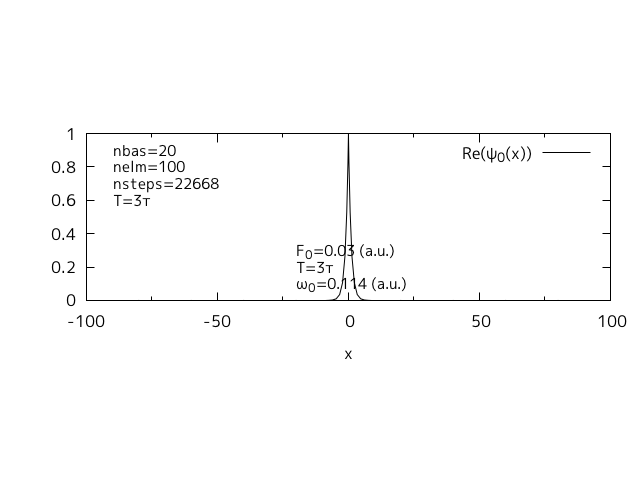
\includegraphics[scale=.20, trim={6 100 0 100},clip]{images/114_f003_3_10_wfc0.png} \\
% 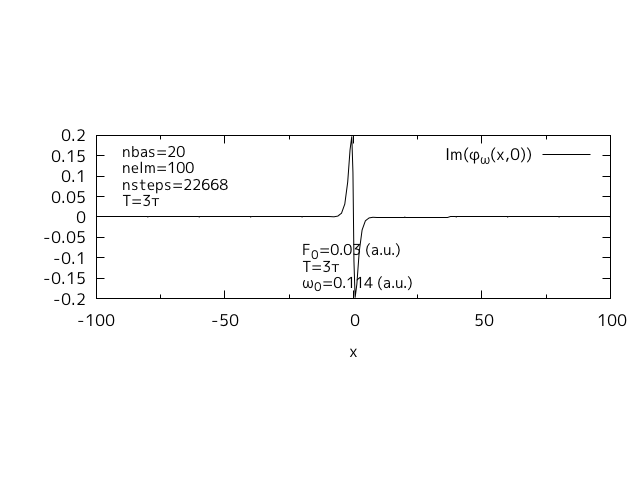
\includegraphics[scale=.20, trim={6 100 0 100},clip]{images/114_f003_3_10_phic0.png} \\
%% \includegraphics[scale=.20, trim={6 130 10 100},clip]{images/114_f003_8_03_hhg.png} 
%%%\caption{Eigenvalues.}
%%\label{fig:pemd_0114}
%\end{figure}
%
%\end{minipage}
%\end{textblock*}
%
%
%\begin{textblock*}{500pt}(130pt,60pt)
%%\centering
%%\rotatebox{90}{
% \begin{minipage}{0.0\linewidth}
% \begin{figure}[tp]
% 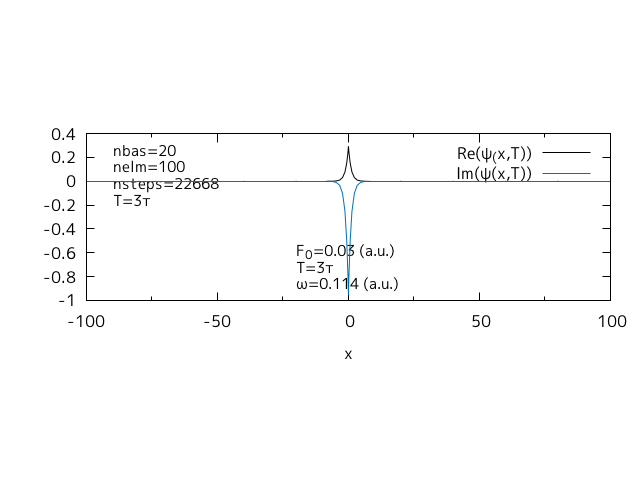
\includegraphics[scale=.20, trim={6 100 0 100},clip]{images/114_f003_3_10_wfc.png} \\
% 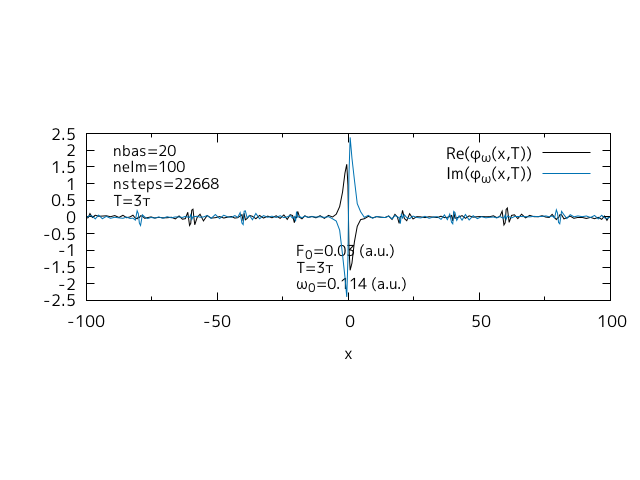
\includegraphics[scale=.20, trim={6 100 0 100},clip]{images/114_f003_3_10_phic.png} \\
%% 
\includegraphics[scale=.20, trim={6 130 10 100},clip]{images/114_f003_12_07_hhg.png} 
%%%\caption{Eigenvalues.}
%%\label{fig:pemd_0114}
% \end{figure}
%
%\end{minipage}
%\end{textblock*}
%
%
%\begin{textblock*}{500pt}(290pt,60pt)
%%\centering
%%\rotatebox{90}{
% \begin{minipage}{0.0\linewidth}
% \begin{figure}[tp]
% 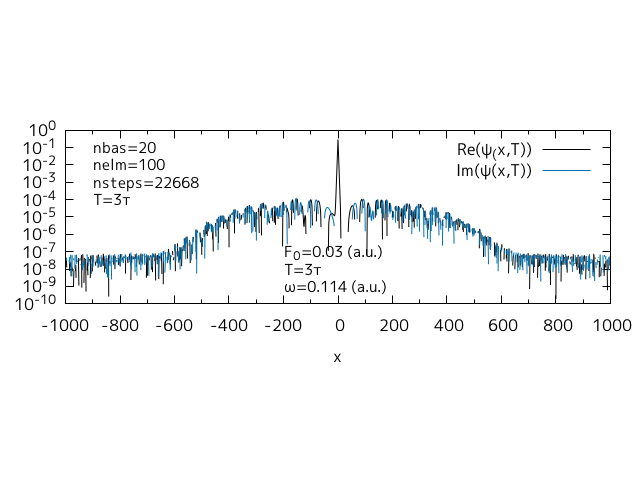
\includegraphics[scale=.20, trim={6 100 0 100},clip]{images/114_f003_3_10_wfc_log.png} \\
% 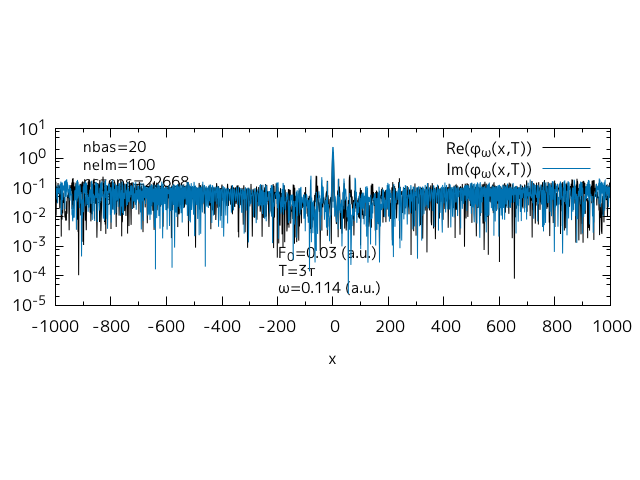
\includegraphics[scale=.20, trim={6 100 0 100},clip]{images/114_f003_3_10_phic_log.png} \\
% 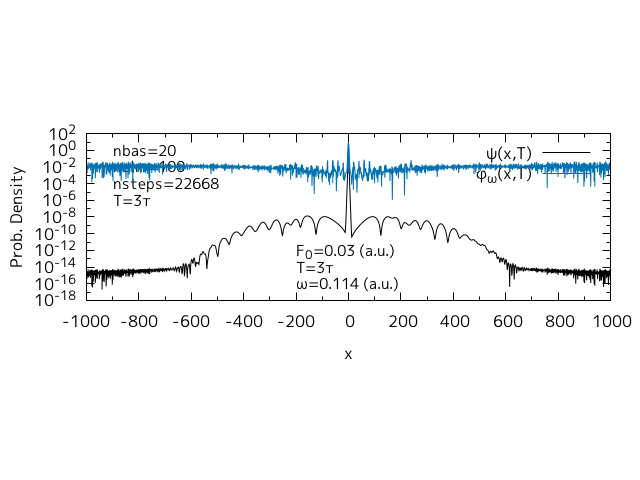
\includegraphics[scale=.20, trim={6 100 0 100},clip]{images/114_f003_3_10_density.png} 
%%%\caption{Eigenvalues.}
%%\label{fig:pemd_0114}
% \end{figure}
%
%\end{minipage}
%\end{textblock*}
%
%
%\begin{textblock*}{50pt}(30pt,180pt)
%\scriptsize
%%\begin{itemize}
%%\item How to deduce the coefficients of $\phi_\nu$?
%\begin{align}
%& {\rm nbas}   = 20                 \nonumber\\
%& {\rm nelm}   = 100                \nonumber\\ 
%& {\rm nsteps} = 22668              \nonumber\\ 
%& {\rm xmax}   = 2000               \nonumber\\ 
%& T = 3\tau                         \nonumber
%\end{align}
%%\end{itemize}
%\end{textblock*}
%
%\end{frame}
%
%
%
%
%
%\begin{frame}
%\frametitle{Quantum theory of radiation by nonstationary systems 
%	with application to high-order harmonic generation
%        (Phys. Rev. A 101, 013410 (2020))}
%	\framesubtitle{The wavefunction $\phi_\omega(x,t) \;\;\;(\omega=1)$}
%
%\begin{textblock*}{500pt}(5pt,60pt)
%%\centering
%%\rotatebox{90}{
% \begin{minipage}{0.0\linewidth}
% \begin{figure}[tp]
% 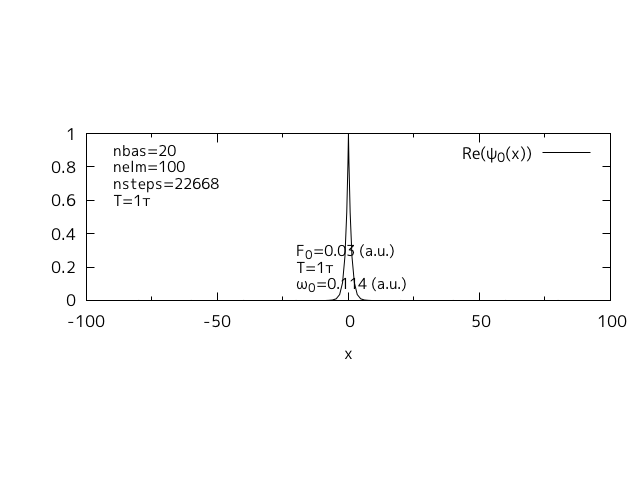
\includegraphics[scale=.20, trim={6 100 0 100},clip]{images/114_f003_1_01_wfc0.png} \\
% 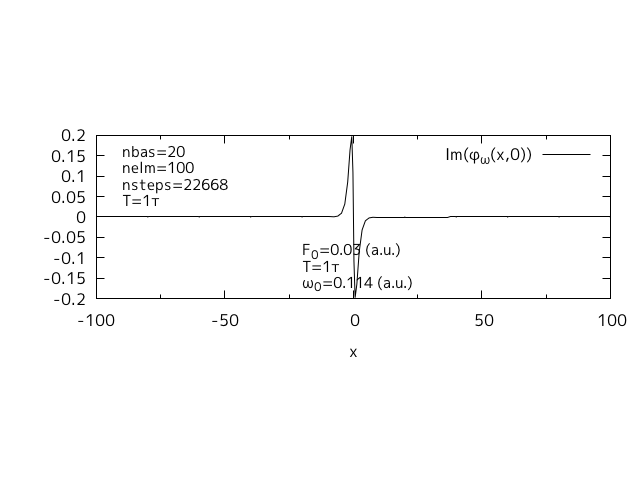
\includegraphics[scale=.20, trim={6 100 0 100},clip]{images/114_f003_1_01_phic0.png} \\
%% \includegraphics[scale=.20, trim={6 130 10 100},clip]{images/114_f003_8_03_hhg.png} 
%%%\caption{Eigenvalues.}
%%\label{fig:pemd_0114}
%\end{figure}
%
%\end{minipage}
%\end{textblock*}
%
%
%\begin{textblock*}{500pt}(130pt,60pt)
%%\centering
%%\rotatebox{90}{
% \begin{minipage}{0.0\linewidth}
% \begin{figure}[tp]
% 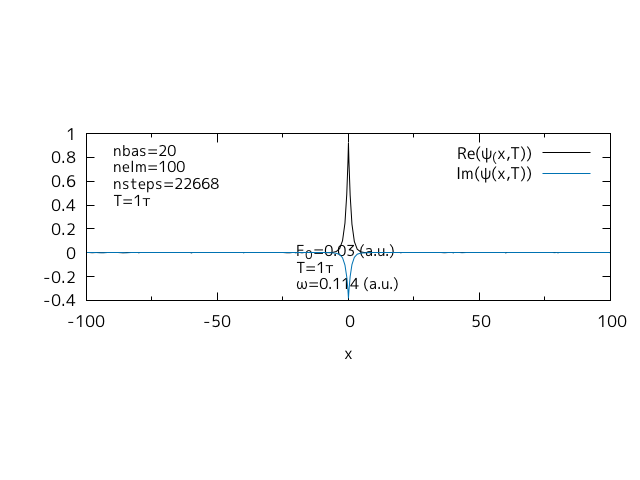
\includegraphics[scale=.20, trim={6 100 0 100},clip]{images/114_f003_1_01_wfc.png} \\
% 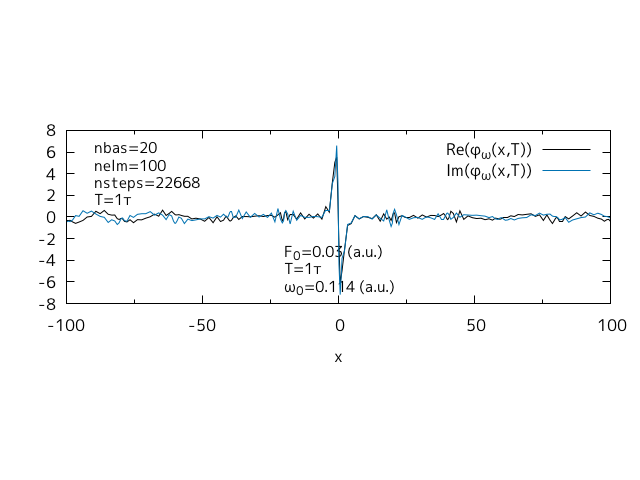
\includegraphics[scale=.20, trim={6 100 0 100},clip]{images/114_f003_1_01_phic.png} \\
%% 
\includegraphics[scale=.20, trim={30 130 10 100},clip]{images/114_f003_12_07_hhg.png} 
%%%\caption{Eigenvalues.}
%%\label{fig:pemd_0114}
% \end{figure}
%
%\end{minipage}
%\end{textblock*}
%
%
%\begin{textblock*}{500pt}(290pt,60pt)
%%\centering
%%\rotatebox{90}{
% \begin{minipage}{0.0\linewidth}
% \begin{figure}[tp]
% 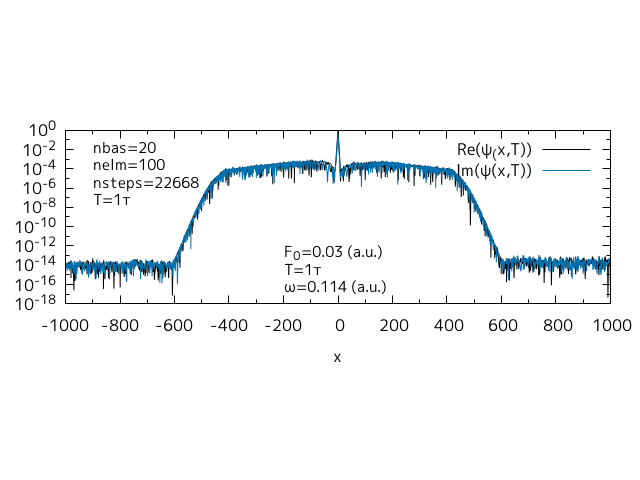
\includegraphics[scale=.20, trim={6 100 0 100},clip]{images/114_f003_1_01_wfc_log.png} \\
% 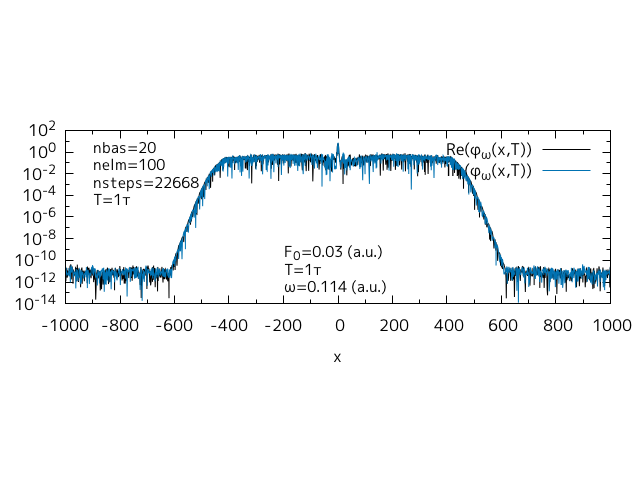
\includegraphics[scale=.20, trim={6 100 0 100},clip]{images/114_f003_1_01_phic_log.png} \\
% 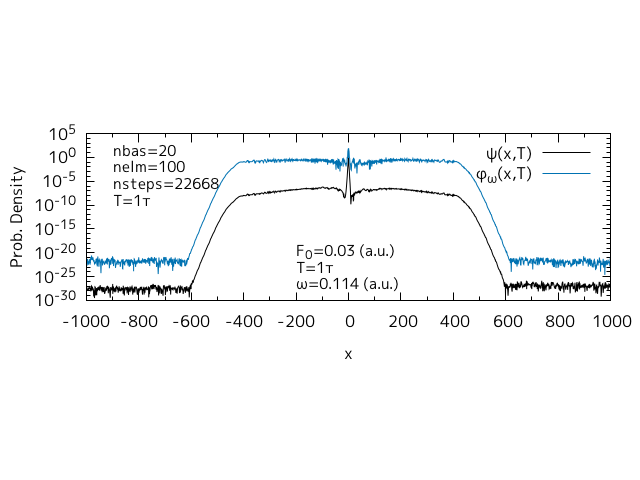
\includegraphics[scale=.20, trim={6 100 0 100},clip]{images/114_f003_1_01_density.png} 
%%%\caption{Eigenvalues.}
%%\label{fig:pemd_0114}
% \end{figure}
%
%\end{minipage}
%\end{textblock*}
%
%
%\begin{textblock*}{50pt}(30pt,180pt)
%\scriptsize
%%\begin{itemize}
%%\item How to deduce the coefficients of $\phi_\nu$?
%\begin{align}
%& {\rm nbas}   = 20                 \nonumber\\
%& {\rm nelm}   = 100                \nonumber\\ 
%& {\rm nsteps} = 22668              \nonumber\\ 
%& {\rm xmax}   = 2000               \nonumber\\ 
%& T = 1\tau                         \nonumber
%\end{align}
%%\end{itemize}
%\end{textblock*}
%
%\end{frame}
%
%
%
%
%
%\begin{frame}
%\frametitle{Quantum theory of radiation by nonstationary systems 
%	with application to high-order harmonic generation
%        (Phys. Rev. A 101, 013410 (2020))}
%	\framesubtitle{About the field}
%
%\begin{textblock*}{500pt}(5pt,60pt)
%%\centering
%%\rotatebox{90}{
% \begin{minipage}{0.0\linewidth}
% \begin{figure}[tp]
% 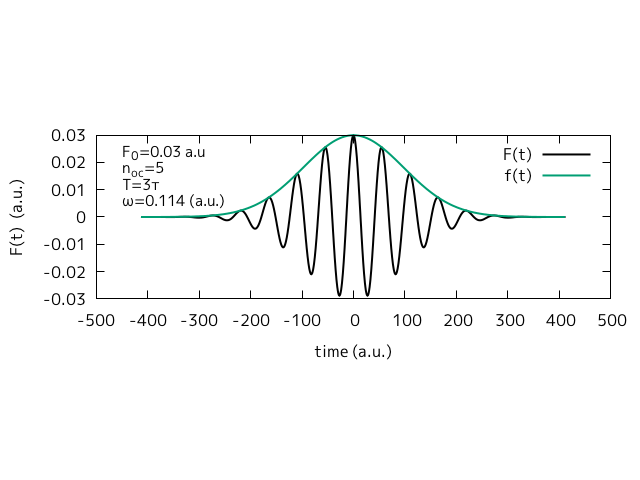
\includegraphics[scale=.20, trim={6 150 10 110},clip]{images/f003_01_114_5_3_field.png} \\
% 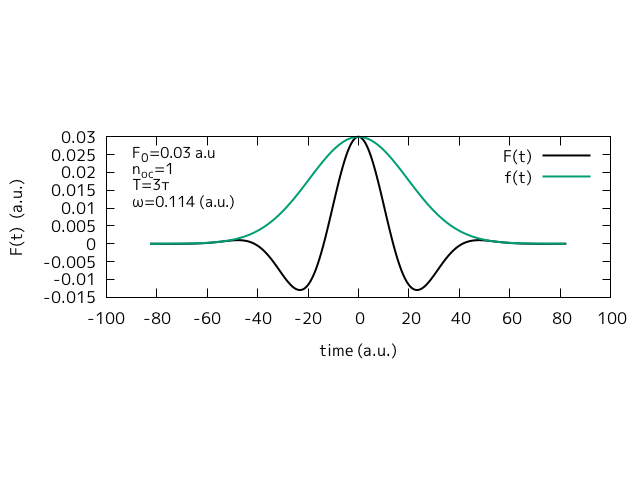
\includegraphics[scale=.20, trim={6 150 10 110},clip]{images/f003_02_114_1_3_field.png} \\
% 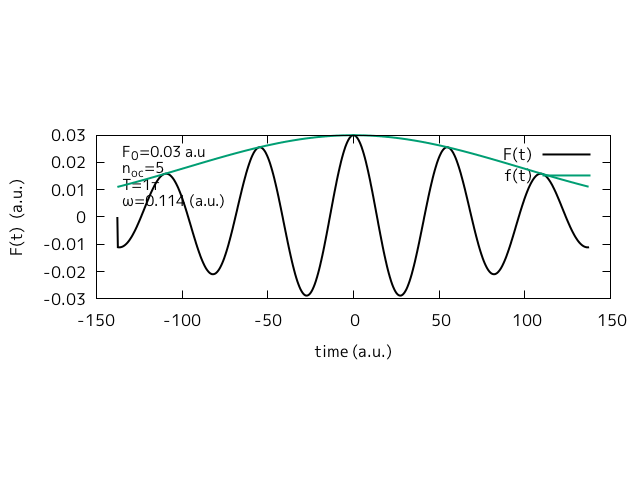
\includegraphics[scale=.20, trim={6 110 10 110},clip]{images/f003_03_114_5_1_field.png} 
%%%\caption{Eigenvalues.}
%%\label{fig:pemd_0114}
%\end{figure}
%
%\end{minipage}
%\end{textblock*}
%
%
%\begin{textblock*}{500pt}(130pt,60pt)
%%\centering
%%\rotatebox{90}{
% \begin{minipage}{0.0\linewidth}
% \begin{figure}[tp]
% 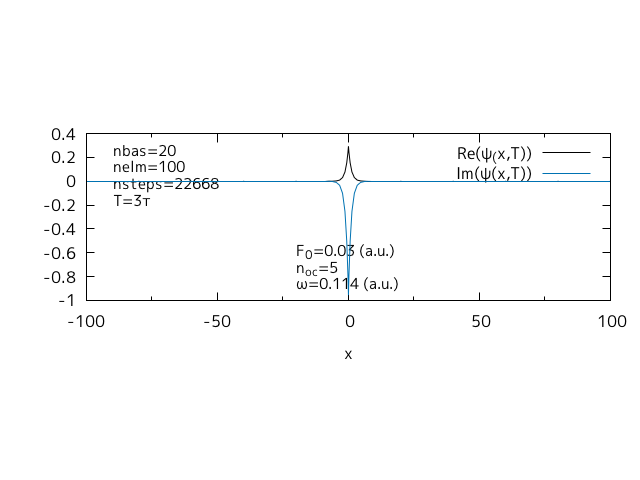
\includegraphics[scale=.20, trim={6 150 10 110},clip]{images/f003_01_114_5_3_wfc.png} \\
% 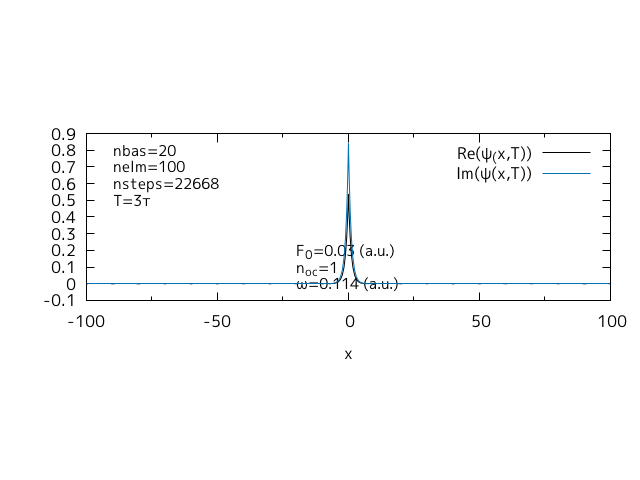
\includegraphics[scale=.20, trim={6 150 10 110},clip]{images/f003_02_114_1_3_wfc.png} \\
% 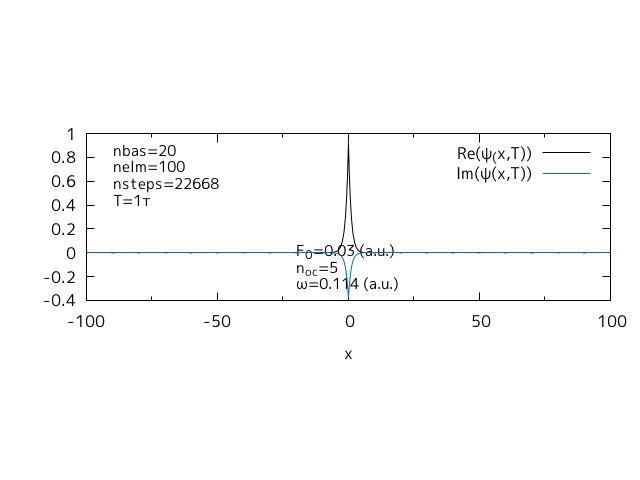
\includegraphics[scale=.20, trim={6 110 10 110},clip]{images/f003_03_114_5_1_wfc.png} 
%%%\caption{Eigenvalues.}
%%\label{fig:pemd_0114}
% \end{figure}
%
%\end{minipage}
%\end{textblock*}
%
%
%\begin{textblock*}{500pt}(290pt,60pt)
%%\centering
%%\rotatebox{90}{
% \begin{minipage}{0.0\linewidth}
% \begin{figure}[tp]
% 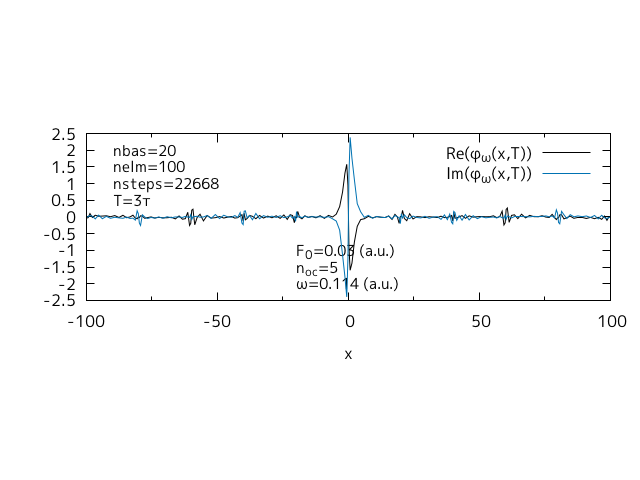
\includegraphics[scale=.20, trim={6 150 10 110},clip]{images/f003_01_114_5_3_phic.png} \\
% 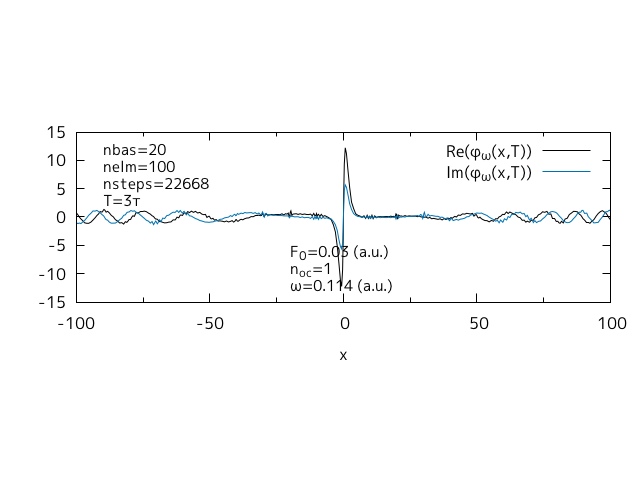
\includegraphics[scale=.20, trim={6 150 10 110},clip]{images/f003_02_114_1_3_phic.png} \\
% 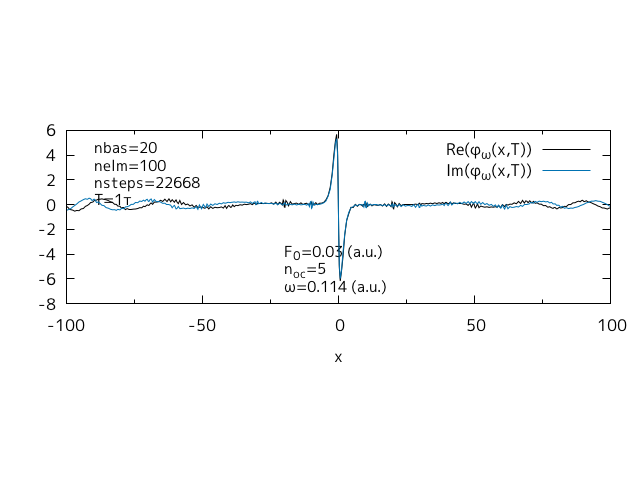
\includegraphics[scale=.20, trim={6 110 10 110},clip]{images/f003_03_114_5_1_phic.png} 
%%%\caption{Eigenvalues.}
%%\label{fig:pemd_0114}
% \end{figure}
%
%\end{minipage}
%\end{textblock*}
%
%
%%\begin{textblock*}{500pt}(360pt,60pt)
%%%\centering
%%%\rotatebox{90}{
%% \begin{minipage}{0.0\linewidth}
%% \begin{figure}[tp]
%% 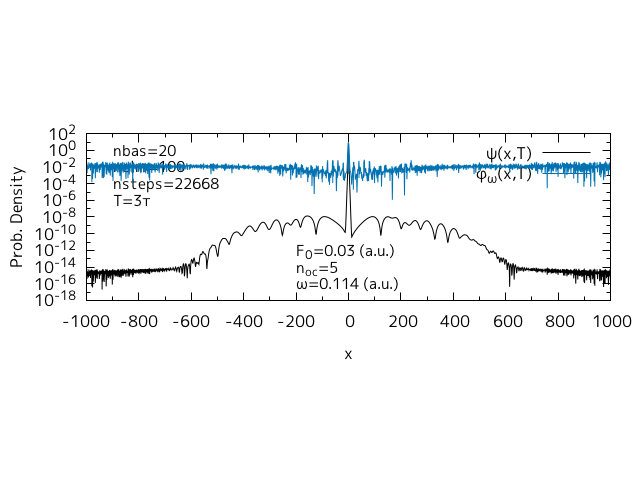
\includegraphics[scale=.20, trim={20 150 10 110},clip]{images/f003_01_114_5_3_density.png} \\
%% 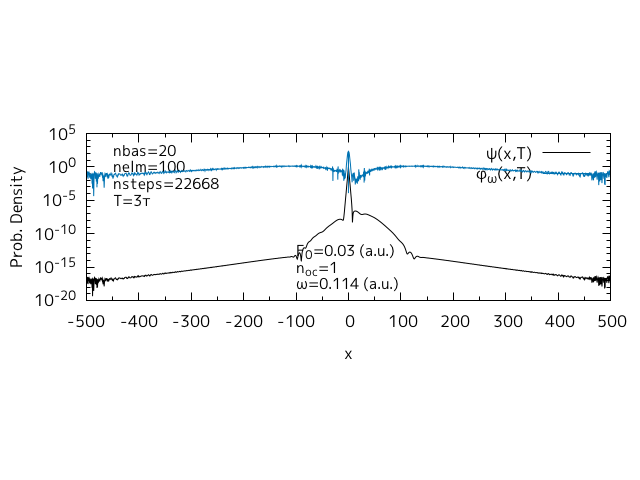
\includegraphics[scale=.20, trim={20 150 10 110},clip]{images/f003_02_114_1_3_density.png} \\
%% 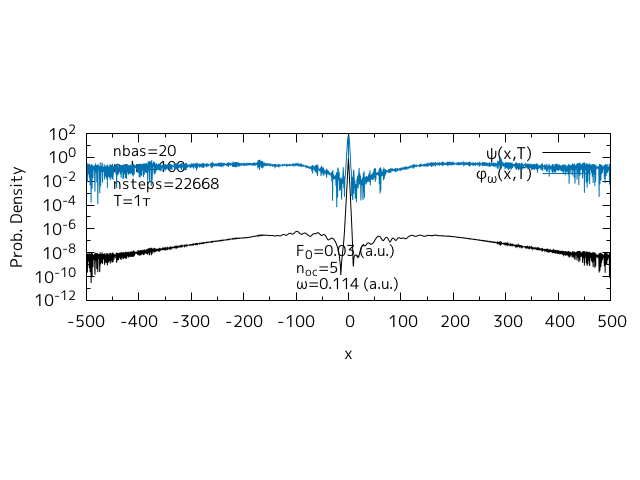
\includegraphics[scale=.20, trim={20 110 10 110},clip]{images/f003_03_114_5_1_density.png} 
%%%%\caption{Eigenvalues.}
%%%\label{fig:pemd_0114}
%% \end{figure}
%%
%%\end{minipage}
%%\end{textblock*}
%
%
%%\begin{textblock*}{50pt}(30pt,180pt)
%%\scriptsize
%%%\begin{itemize}
%%\begin{align}
%%& {\rm nbas}   = 40                 \nonumber\\
%%& {\rm nelm}   = 200                \nonumber\\ 
%%& {\rm nsteps} = 22668              \nonumber\\ 
%%& {\rm xmax}   = 4000               \nonumber\\ 
%%& T = 3\tau                         \nonumber
%%\end{align}
%%%\end{itemize}
%%\end{textblock*}
%
%\end{frame}





\begin{frame}
\frametitle{Quantum theory of radiation by nonstationary systems 
	with application to high-order harmonic generation
        (Phys. Rev. A 101, 013410 (2020))}
	\framesubtitle{The FEDVR basis - 1 - basic properties}


\begin{textblock*}{400pt}(30pt,60pt)
\footnotesize
\begin{itemize}
\item From Ohmi \textit{et al}, Phys, Rev. A 92 (2015), we get
\begin{align}
& \pi_i^s (r) = \frac{1}{\sqrt{\omega_i}} 
       \prod_{\substack{k=1 \\ k\neq i}}^{N_p}
       \frac{r-r_k^s}{r_i^s - r_k^s}, \hspace{50pt} 
    \pi_i^s(r_k^s) = \delta_{ik}/\sqrt{\omega_i^s},  \\
& \left.\frac{d\pi_i^s (r)}{dr}\right|_{r=r_j^s} 
       =  \frac{1}{\sqrt{\omega_i}} \left\lbrace
      \begin{array}{l} 
       \frac{1}{r_i^s - r_j^s}\prod_{\substack{k=1 \\ k\neq i,j}}^{N_p}
       \frac{r_j^s - r_k^s}{r_i^s - r_k^s}, \hspace{50pt} i \neq j, \\
       \frac{1}{2}\left(\Big[\pi_i^s(r_{N_p}^s)\Big]^2 
       - \Big[\pi_i^s(r_1^s)\Big]^2\right), \hspace{20pt} i=j,
\end{array}\right. \label{eqn:diff_dvr_basis_nodes}
\end{align}

\item $N_s$ sectors $r_0 \leqslant  \ldots r_s \leqslant r_{N_s}$
and $N_p$ nodes a sector, which makes the number of point $N$ so
\begin{align}
N & = N_s(N_p-1) + 1     \\
n & = (s-1)(N_p-1) + i
\end{align}

with
\begin{equation}
i = 1, \ldots, N_p,\hspace{20pt}
s = 1, \ldots, N_s, \hspace{20pt}
n = 1, \ldots, N    \nonumber
\end{equation}

\end{itemize}
\end{textblock*}

\end{frame}




\begin{frame}
\frametitle{Quantum theory of radiation by nonstationary systems 
	with application to high-order harmonic generation
        (Phys. Rev. A 101, 013410 (2020))}
	\framesubtitle{The FEDVR basis - 2 - The global basis}


\begin{textblock*}{400pt}(30pt,60pt)
\footnotesize
\begin{itemize}
\item The global FEDVR basis is defined, for $n = (s-1)(N_p-1)+N_p$,
with $s=1,...,N_s-1$
\begin{align}
& \Pi_n(r)  =  \frac{1}{\sqrt{\Omega_n}}
      \left\lbrace
      \begin{array}{l} 
       \sqrt{\omega_{N_p}^s}\pi_{N_p}^s(r),  
          \hspace{20pt} r \in \left[ r_{s-1}, r_s \right], \\
       \sqrt{\omega_{1}^{s+1}}\pi_{1}^{s+1}(r),  
          \hspace{20pt} r \in \left[ r_{s}, r_{s+1} \right],
      \end{array}\right.
       \hspace{20pt} \Omega_n = \omega_{N_p}^s + \omega_1^{s+1}, 
%     \end{array}\right.,  \hspace{20pt} \Pi_n(r) = \pi_i^s(r), \hspace{10pt} 
%      \hspace{20pt} r \in \left[ r_{s}, r_{s+1} \right]
\label{eqn:global_dvr_basis}
\end{align}

This function bridges the sectors $s$ and $s+1$ and is continuous through the boundary between them (but its derivative is not). 

\item For the other values of $n$
corresponding to the quadrature points inside sectors, i.e.
\begin{equation}
n = (s-1)(N_p-1)+i
\end{equation}
and at the outer boundary $r_N = r_m$ of the box, we have

\begin{align}
       \Pi_n(r) = \pi_i^s(r), \hspace{10pt} 
         \hspace{20pt} r & \in \left[ r_{s}, r_{s+1} \right],
       \hspace{30pt} \Omega_n = \omega_i^s, \\
       \Pi_n(r_{n^\prime}) & = \delta_{nn^\prime} / \sqrt{\Omega_n}, \\
       \int_0^{r_m} \Pi_n(r) f(r) & \Pi_{n^\prime}(r) dr \sim f(r_n)\delta_{nn^\prime}.
\end{align}



%\begin{equation}
%\psi(x,t) = \sum_{n=1}^{N} c_{n}(t)\Pi_n(x)
%\hspace{10pt} \Longrightarrow  \hspace{10pt}
%\frac{d}{dx}\psi(x,t) = \sum_{n=1}^{N} c_{n}(t)
%   \frac{d}{dx}\Pi_n(x)
%\end{equation}
%
%In particular, 
%\begin{equation}
%\psi(x,0) = \sum_{n=1}^{N} c_{n}(0)\Pi_n(x)
%\hspace{10pt} \Longrightarrow  \hspace{10pt}
%\frac{d}{dx}\psi(x,0) = \sum_{n=1}^{N} c_{n}(0)
%   \frac{d}{dx}\Pi_n(x)
%\end{equation}

\end{itemize}

\end{textblock*}



\end{frame}



\begin{frame}
\frametitle{Quantum theory of radiation by nonstationary systems 
	with application to high-order harmonic generation
        (Phys. Rev. A 101, 013410 (2020))}
	\framesubtitle{The FEDVR basis - 3 - the derivative}


\begin{textblock*}{400pt}(30pt,60pt)
\footnotesize
\begin{itemize}
\item We can extend Eq. (\ref{eqn:diff_dvr_basis_nodes}) to any $r$
of the domain and write
\begin{align}
%& \frac{d\pi_i^s (r)}{dr}
%       =  \frac{1}{\sqrt{\omega_i^s}} \sum_{\substack{k=1 \\ k\neq i}}^{N_p} 
%       \frac{1}{r_i^s - r_k^s}\prod_{\substack{j=1 \\ j\neq k,i}}^{N_p}
%       \frac{r - r_j^s}{r_i^s - r_j^s},
%\label{eqn:diff_dvr_basis}
& \frac{d\pi_i^s (r)}{dr}
       =  \frac{1}{\sqrt{\omega_i^s}} \sum_{\substack{j=1 \\ j\neq i}}^{N_p} 
       \frac{1}{r_i^s - r_j^s}\prod_{\substack{k=1 \\ k\neq j,i}}^{N_p}
       \frac{r - r_k^s}{r_i^s - r_k^s},
\label{eqn:diff_dvr_basis}
\end{align}

\item In terms of $\Pi_n$, the derivative is expressed as,
for $n = (s-1)(N_p-1) + N_p$, 
with $\Omega_n = \omega_{N_p}^s + \omega_1^{s+1}$

\begin{align}
& \frac{d\Pi_n(r)}{dr}
=  \frac{1}{\sqrt{\Omega_n}}
      \left\lbrace
         \begin{array}{l} 
       \sqrt{\omega_{N_p}^s}\,d\pi_{N_p}^s(r)/dr,  
          \hspace{10pt} \ r \leqslant r_s, \hspace{10pt} \\
       \sqrt{\omega_{1}^{s+1}}\,d\pi_{1}^{s+1}(r)/dr,  
          \hspace{10pt} r \geqslant  r_{s}, \hspace{10pt}
         \end{array}\right.
\end{align}

\noindent and reduced to (\ref{eqn:diff_dvr_basis}) otherwise.

The quantities we are looking for are, with the proper normalization

\begin{align}
&\psi(x,t) = \sum_{n=1}^{N} \sqrt{\omega^s_i}
          c_n(t)\Pi_n(x), \hspace{50pt} \mbox{ and }
&\frac{d}{dx}\psi(x,t) = \sum_{n=1}^{N} \sqrt{\omega^s_i}
         c_n(t) \frac{d}{dx}\Pi_n(x).
\label{eqn:wf_dwf}
\end{align}


%\item For $n = (s-1)(N_p-1)+N_p$
%and $N_p$ nodes a sector, which makes the number of point $N$ so
%\begin{align}
%N & = N_s(N_p-1) + 1     \\
%n & = (s-1)(N_p-1) + i \\
%\end{align}
%
%%with
%%\begin{equation}
%%i = 1, \ldots, N_p,\hspace{20pt}
%%s = 1, \ldots, N_s, \hspace{20pt}
%%n = 1, \ldots, N    \nonumber
%%\end{equation}

\end{itemize}
\end{textblock*}

\end{frame}






\begin{frame}
\frametitle{Quantum theory of radiation by nonstationary systems 
	with application to high-order harmonic generation
        (Phys. Rev. A 101, 013410 (2020))}
	\framesubtitle{The FEDVR basis - The nodes}

%\begin{textblock*}{100pt}(5pt,60pt)
%%\centering
%%\rotatebox{90}{
% \begin{minipage}{0.0\linewidth}
% \begin{figure}[tp]
% 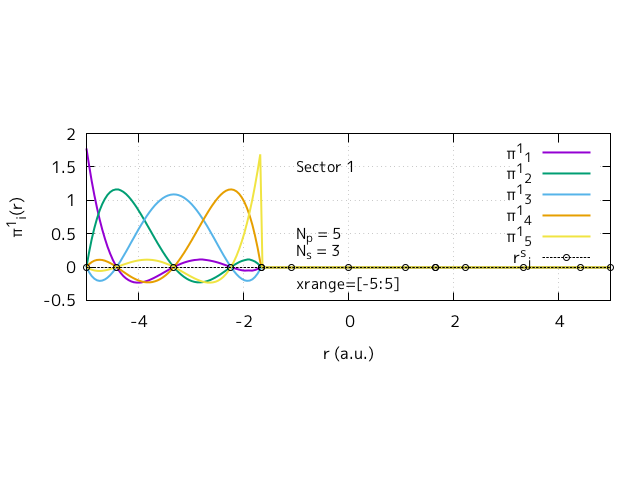
\includegraphics[scale=.20, trim={6 150 10 110},clip]{images/fedvr_sect1.png} \\
%  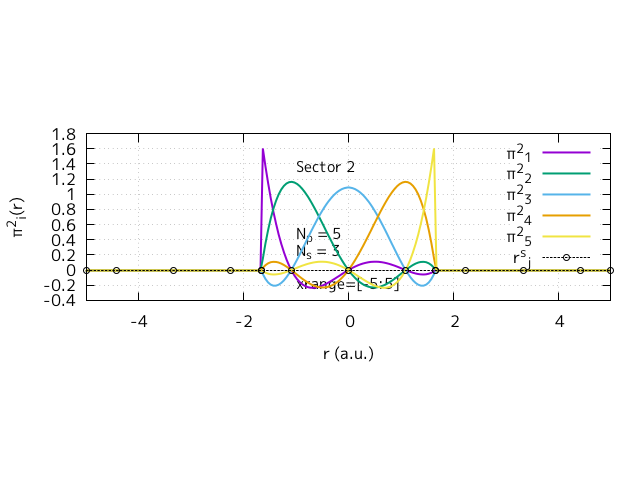
\includegraphics[scale=.20, trim={6 150 10 110},clip]{images/fedvr_sect2.png} \\
%  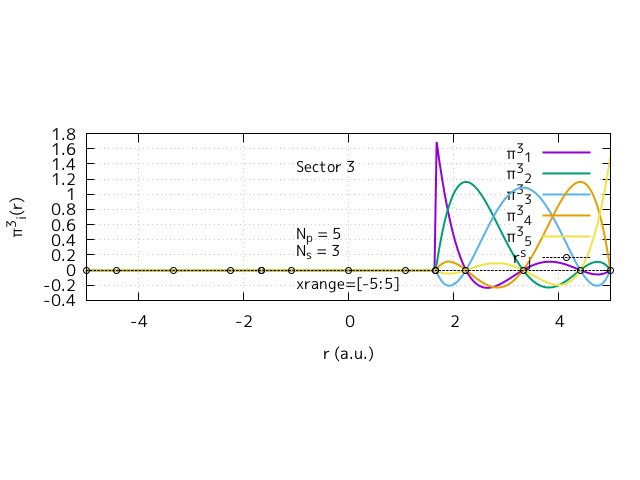
\includegraphics[scale=.20, trim={6 110 10 110},clip]{images/fedvr_sect3.png} 
%%%%\caption{Eigenvalues.}
%%\label{fig:pemd_0114}
%\end{figure}
%
%\end{minipage}
%\end{textblock*}


\begin{textblock*}{\linewidth}(90pt,60pt)
\rotatebox{0}{
\begin{minipage}{\linewidth}
{
\Tiny
\centering
\input{tables/rk_4_5.tab}
}
\end{minipage}
}
\end{textblock*}



\begin{textblock*}{150pt}(20pt,70pt)
\tiny

\begin{align}
& N_s = 4,\ N_p = 5, \hspace{20pt} N = 15,\;\; N^\prime = 17. \nonumber\\
& n^\prime = (s-1)(N_p-1)+i \nonumber\\
& N = N_s (N_p - 1) - 1, \hspace{10pt} N = 15 \nonumber \\
& N^\prime = N_s (N_p - 1) + 1 \hspace{10pt} N^\prime = 17. \nonumber
\end{align}
\footnotesize
\begin{itemize}
\item $\mathcal{B}^\prime$ provides mathematical support
\item $\mathcal{B}$ is where we have the expression of the wavefunction
\item We note that $n^\prime = n +1$ when defined
\end{itemize}

\end{textblock*}
\end{frame}




\begin{frame}
\frametitle{Quantum theory of radiation by nonstationary systems 
	with application to high-order harmonic generation
        (Phys. Rev. A 101, 013410 (2020))}
	\framesubtitle{The FEDVR basis - $\Pi_n$ and its derivative}

\begin{textblock*}{100pt}(5pt,60pt)
%\centering
%\rotatebox{90}{
 \begin{minipage}{0.0\linewidth}
 \begin{figure}[tp]
 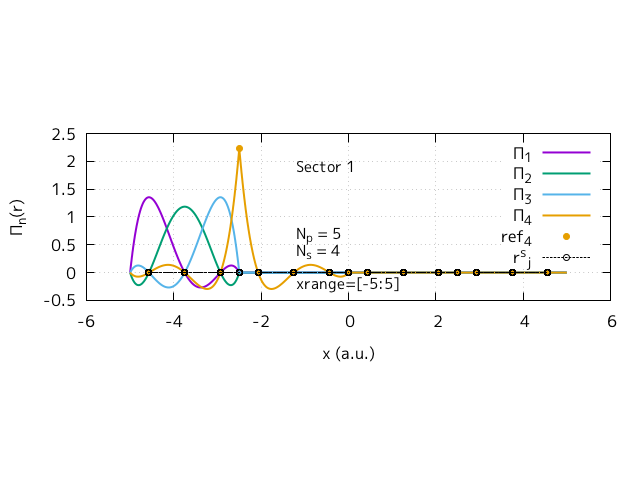
\includegraphics[scale=.20, trim={6 150 10 110},clip]{images/fedvr_sect1_g_pis_all.png} \\
  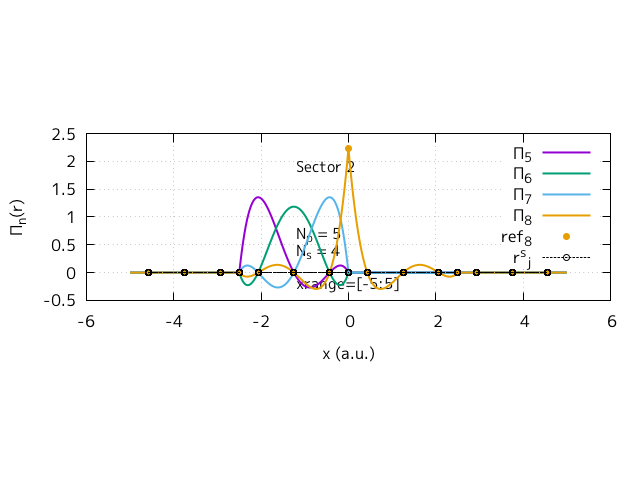
\includegraphics[scale=.20, trim={6 150 10 110},clip]{images/fedvr_sect2_g_pis_all.png} \\
  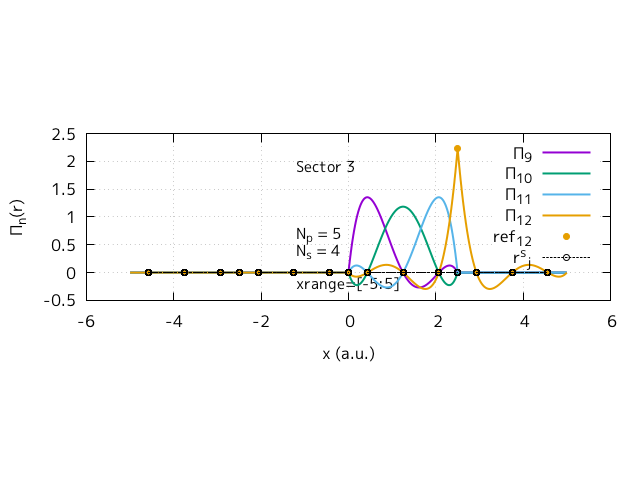
\includegraphics[scale=.20, trim={6 150 10 110},clip]{images/fedvr_sect3_g_pis_all.png} 
  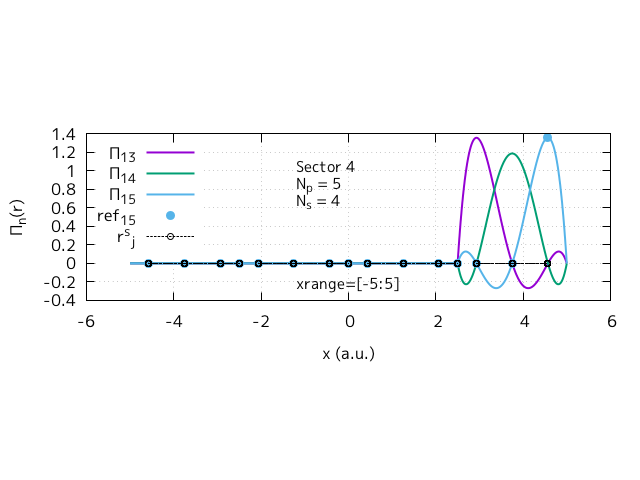
\includegraphics[scale=.20, trim={6 110 10 110},clip]{images/fedvr_sect4_g_pis_all.png} 
%%%\caption{Eigenvalues.}
%\label{fig:pemd_0114}
\end{figure}

\end{minipage}
\end{textblock*}


\begin{textblock*}{100pt}(130pt,60pt)
%\centering
%\rotatebox{90}{
 \begin{minipage}{0.0\linewidth}
 \begin{figure}[tp]
 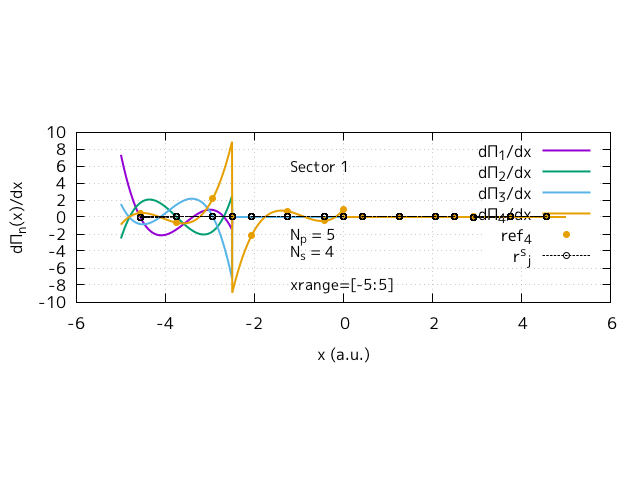
\includegraphics[scale=.20, trim={6 150 10 110},clip]{images/fedvr_sect1_dg_pis_all.png} \\
  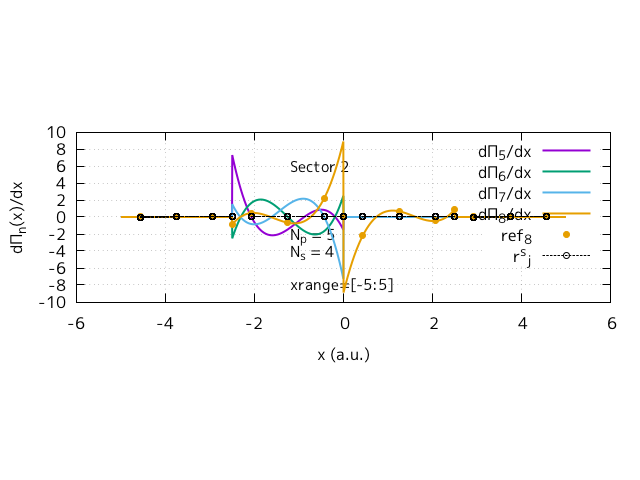
\includegraphics[scale=.20, trim={6 150 10 110},clip]{images/fedvr_sect2_dg_pis_all.png} \\
  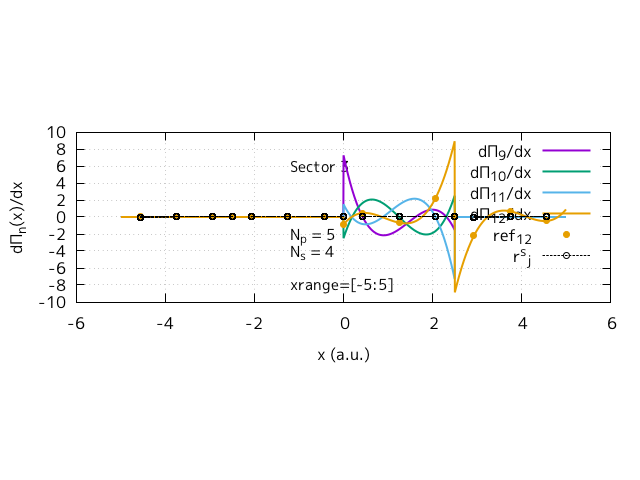
\includegraphics[scale=.20, trim={6 150 10 110},clip]{images/fedvr_sect3_dg_pis_all.png} 
  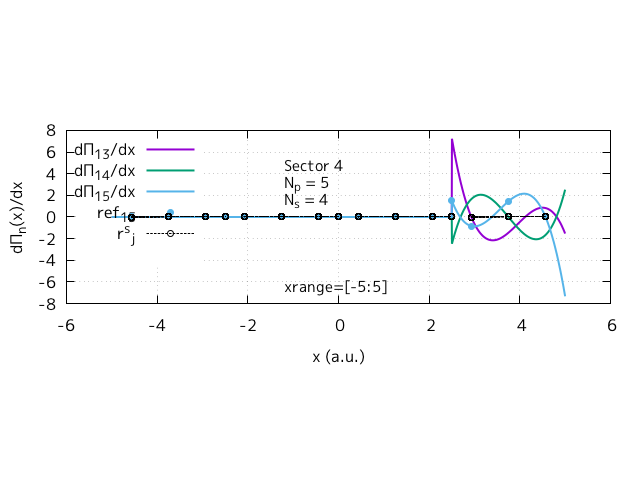
\includegraphics[scale=.20, trim={6 110 10 110},clip]{images/fedvr_sect4_dg_pis_all.png} 
%%%\caption{Eigenvalues.}
%\label{fig:pemd_0114}
\end{figure}

\end{minipage}
\end{textblock*}


%\begin{textblock*}{100pt}(255pt,60pt)
%%\centering
%%\rotatebox{90}{
% \begin{minipage}{0.0\linewidth}
% \begin{figure}[tp]
% 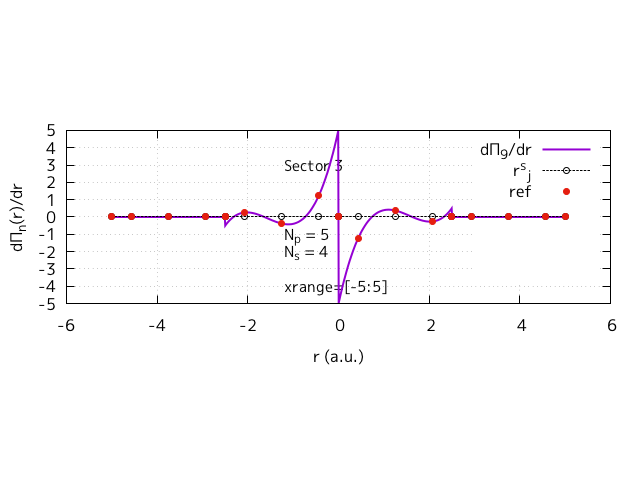
\includegraphics[scale=.20, trim={6 150 10 110},clip]{images/fedvr_sect3_dpi_diff_1.png} \\
%  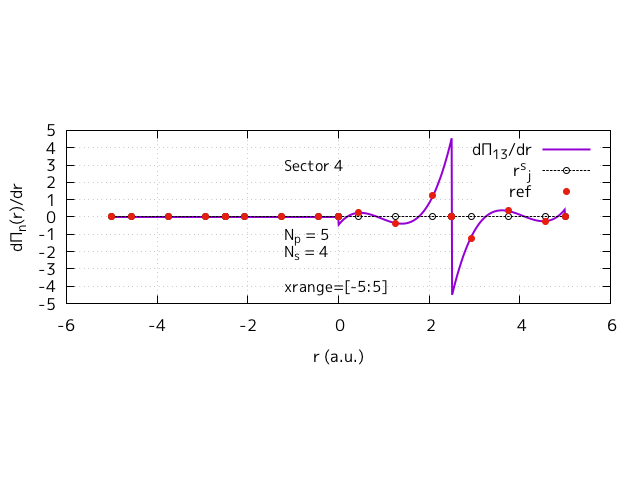
\includegraphics[scale=.20, trim={6 150 10 110},clip]{images/fedvr_sect4_dpi_diff_1.png} \\
%% 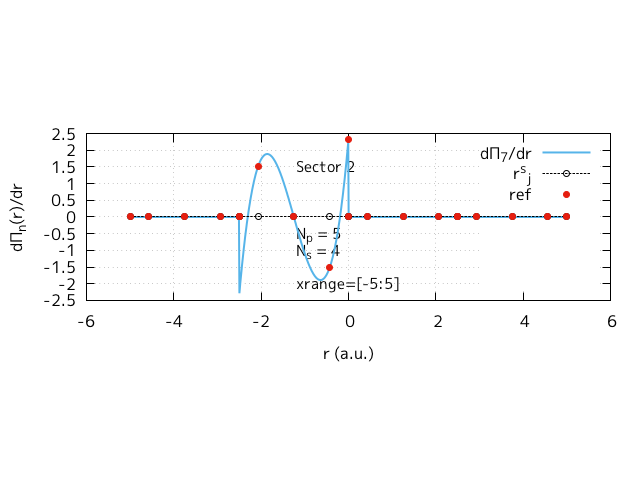
\includegraphics[scale=.20, trim={6 150 10 110},clip]{images/fedvr_sect2_dpi_diff_3.png} 
%% 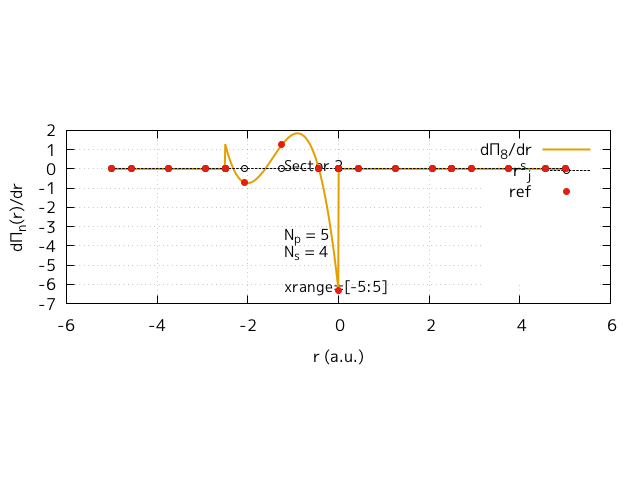
\includegraphics[scale=.20, trim={6 110 10 110},clip]{images/fedvr_sect2_dpi_diff_4.png} 
%%%%\caption{Eigenvalues.}
%%\label{fig:pemd_0114}
%\end{figure}
%
%\end{minipage}
%\end{textblock*}


%\begin{textblock*}{\linewidth}(90pt,60pt)
%\rotatebox{0}{
%\begin{minipage}{\linewidth}
%{
%\Tiny
%\centering
%\input{tables/rk_4_5.tab}
%}
%\end{minipage}
%}
%\end{textblock*}



\begin{textblock*}{170pt}(260pt,100pt)

\footnotesize

\begin{align}
& \Pi_{n}(x) = \sum_{m=1}^{N}\Pi_n(x_{m}) 
   {\boldsymbol{\hat{e}}}_m  \label{eqn:discrete_points}
\end{align}


\tiny

\begin{itemize}
\item The continuous line represent Eq. (\ref{eqn:global_dvr_basis})
for an arbitrary $x$ in the sector's range
\item The colored dot represents the value 
for the different nodes  
$x_j$, i.e. Eq. (\ref{eqn:discrete_points}), with $\boldsymbol{\hat{e}}_m$
the unitary vectors of the cartesian basis


\end{itemize}

\end{textblock*}
\end{frame}



%\begin{frame}
%\frametitle{Quantum theory of radiation by nonstationary systems 
%	with application to high-order harmonic generation
%        (Phys. Rev. A 101, 013410 (2020))}
%	\framesubtitle{The FEDVR basis - The wavefunction and its derivative}
%
%\begin{textblock*}{100pt}(5pt,60pt)
%%\centering
%%\rotatebox{90}{
% \begin{minipage}{0.0\linewidth}
% \begin{figure}[tp]
% 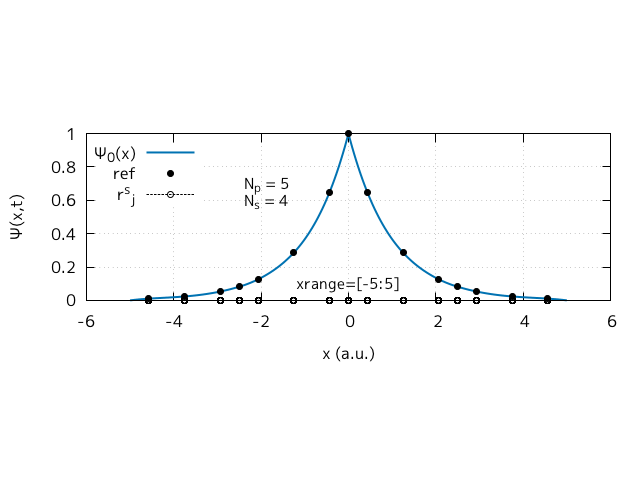
\includegraphics[scale=.20, trim={6 150 10 110},clip]{images/fedvr_wavefunc_.png} \\
%  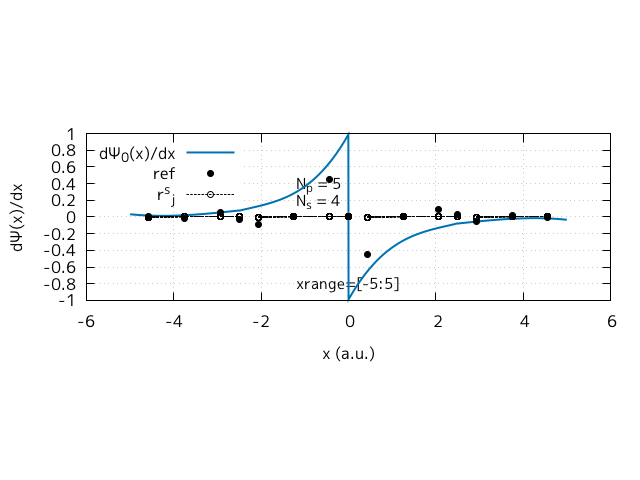
\includegraphics[scale=.20, trim={6 150 10 110},clip]{images/fedvr_deriv_wavefunc_1.png} \\
%%%%\caption{Eigenvalues.}
%%\label{fig:pemd_0114}
%\end{figure}
%
%\end{minipage}
%\end{textblock*}
%
%
%%\begin{textblock*}{100pt}(130pt,60pt)
%%%\centering
%%%\rotatebox{90}{
%% \begin{minipage}{0.0\linewidth}
%% \begin{figure}[tp]
%% 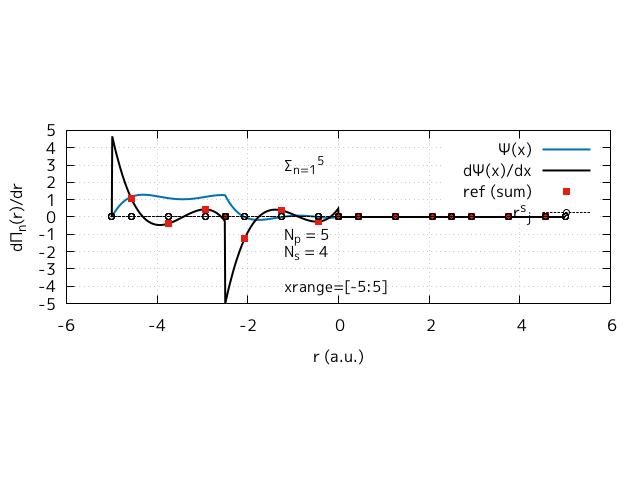
\includegraphics[scale=.20, trim={6 150 10 110},clip]{images/fedvr_sect1_dpi_diff_test_5.png} \\
%%  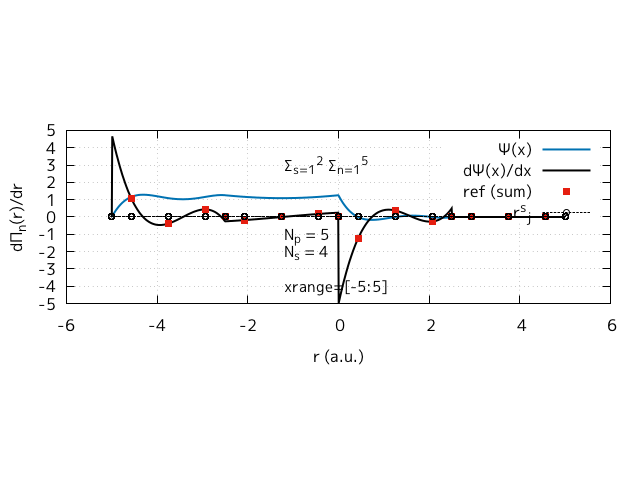
\includegraphics[scale=.20, trim={6 150 10 110},clip]{images/fedvr_sect2_dpi_diff_test_5.png} \\
%%  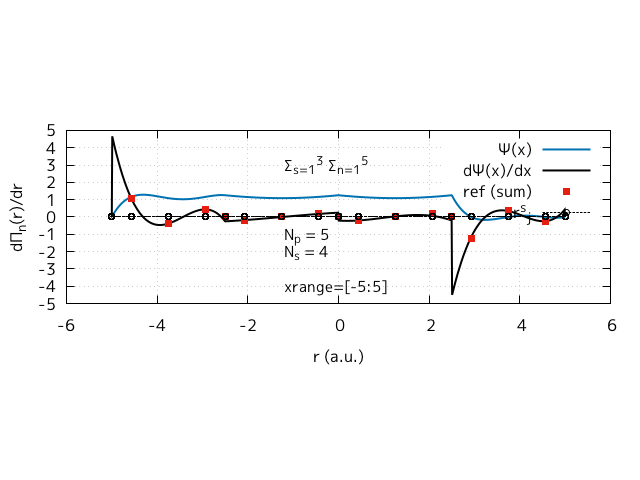
\includegraphics[scale=.20, trim={6 150 10 110},clip]{images/fedvr_sect3_dpi_diff_test_5.png} 
%%  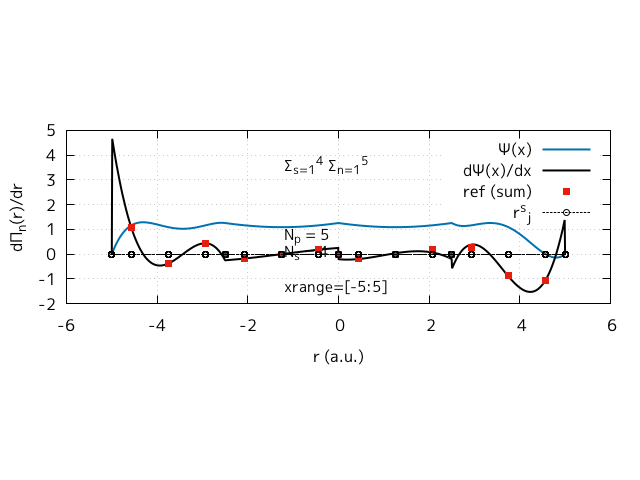
\includegraphics[scale=.20, trim={6 110 10 110},clip]{images/fedvr_sect4_dpi_diff_test_5.png} 
%%%%%\caption{Eigenvalues.}
%%%\label{fig:pemd_0114}
%%\end{figure}
%%
%%\end{minipage}
%%\end{textblock*}
%%
%%
%%%\begin{textblock*}{100pt}(255pt,60pt)
%%%%\centering
%%%%\rotatebox{90}{
%%% \begin{minipage}{0.0\linewidth}
%%% \begin{figure}[tp]
%%% 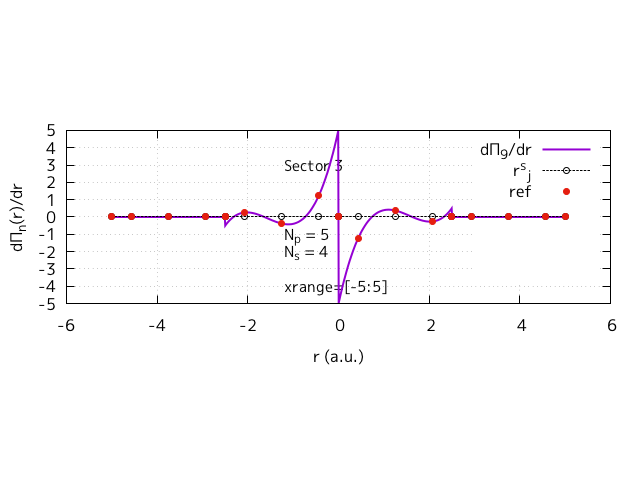
\includegraphics[scale=.20, trim={6 150 10 110},clip]{images/fedvr_sect3_dpi_diff_1.png} \\
%%%  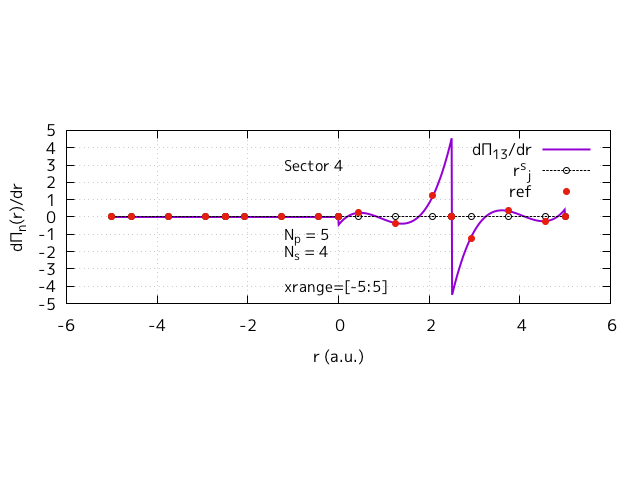
\includegraphics[scale=.20, trim={6 150 10 110},clip]{images/fedvr_sect4_dpi_diff_1.png} \\
%%%% 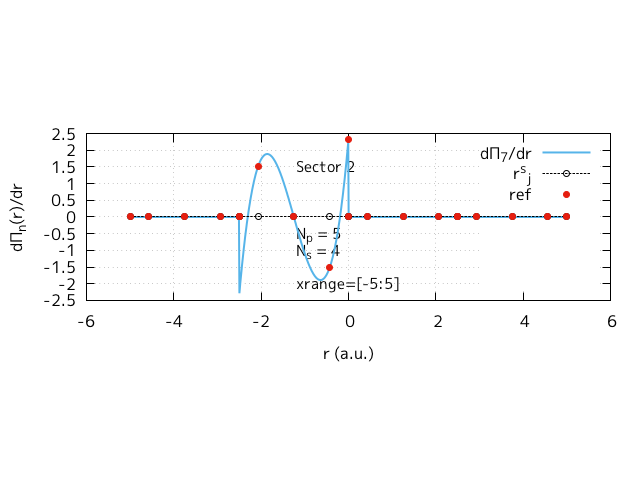
\includegraphics[scale=.20, trim={6 150 10 110},clip]{images/fedvr_sect2_dpi_diff_3.png} 
%%%% 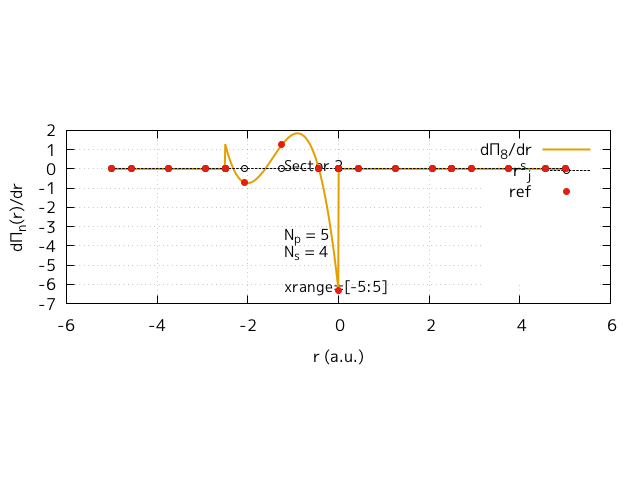
\includegraphics[scale=.20, trim={6 110 10 110},clip]{images/fedvr_sect2_dpi_diff_4.png} 
%%%%%%\caption{Eigenvalues.}
%%%%\label{fig:pemd_0114}
%%%\end{figure}
%%%
%%%\end{minipage}
%%%\end{textblock*}
%%
%%
%%%\begin{textblock*}{\linewidth}(90pt,60pt)
%%%\rotatebox{0}{
%%%\begin{minipage}{\linewidth}
%%%{
%%%\Tiny
%%%\centering
%%%\input{tables/rk_4_5.tab}
%%%}
%%%\end{minipage}
%%%}
%%%\end{textblock*}
%
%
%
%\begin{textblock*}{200pt}(260pt,100pt)
%\footnotesize
%\begin{align}
%& \Pi_{n}(x) = \sum_{m=1}^{N}\Pi_n(x_{m}) 
%   {\boldsymbol{\hat{e}}}_m \nonumber\\
%& \psi(x,t) = \sum_{n=1}^{N} 
%c_{n}(t)\Pi_{n}(x), \nonumber\\
%& \frac{d}{dx}\psi(x,t) = \sum_{n^\prime=1}^{N} 
%      c_{n}(t)\frac{d}{dx}\Pi_{n}(x). \nonumber
%\end{align}
%\begin{itemize}
%\item We try to model (\ref{eqn:wf_dwf})
%\end{itemize}
%
%\end{textblock*}
%\end{frame}


\begin{frame}
\frametitle{Quantum theory of radiation by nonstationary systems 
	with application to high-order harmonic generation
        (Phys. Rev. A 101, 013410 (2020))}
	\framesubtitle{The FEDVR basis - The analytical wavefunction}

\begin{textblock*}{100pt}(5pt,60pt)
%\centering
%\rotatebox{90}{
 \begin{minipage}{0.0\linewidth}
 \begin{figure}[tp]
 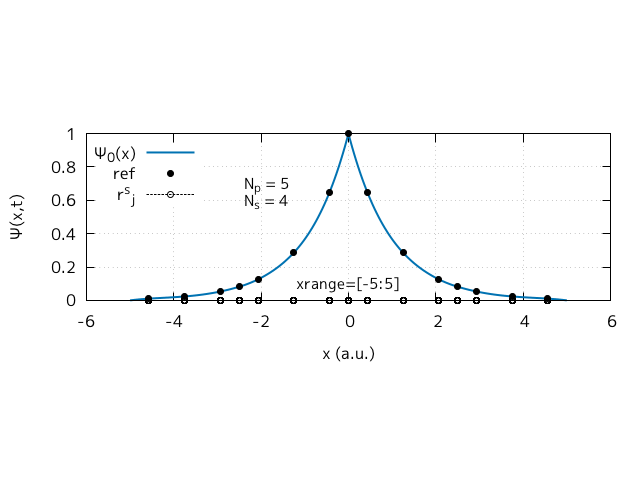
\includegraphics[scale=.22, trim={6 150 10 110},clip]{images/fedvr_wavefunc_.png} \\
%  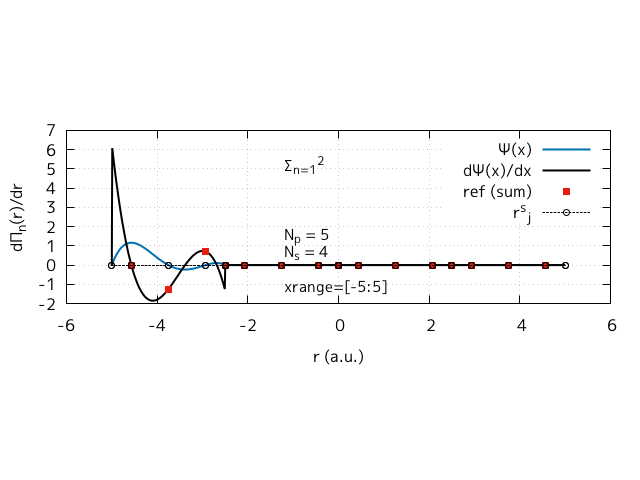
\includegraphics[scale=.20, trim={6 150 10 110},clip]{images/fedvr_sect1_dpi_diff_test_2.png} \\
%  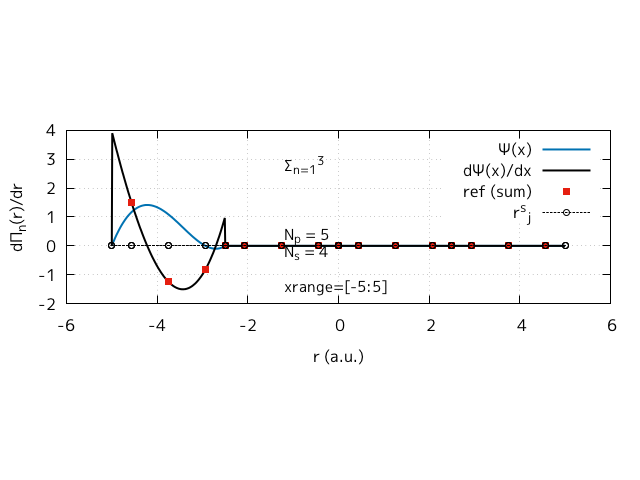
\includegraphics[scale=.20, trim={6 150 10 110},clip]{images/fedvr_sect1_dpi_diff_test_3.png} 
%  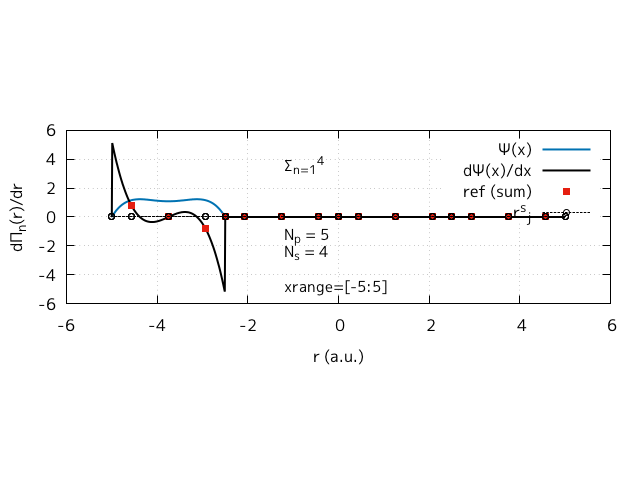
\includegraphics[scale=.20, trim={6 110 10 110},clip]{images/fedvr_sect1_dpi_diff_test_4.png} 
%%%\caption{Eigenvalues.}
%\label{fig:pemd_0114}
\end{figure}

\end{minipage}
\end{textblock*}



\begin{textblock*}{300pt}(150pt,60pt)
\footnotesize

\begin{align}
& \pi_i^s (r) = \frac{1}{\sqrt{\omega_i}} 
       \prod_{\substack{k=1 \\ k\neq i}}^{N_p}
       \frac{r-r_k^s}{r_i^s - r_k^s}, \hspace{50pt} 
    \pi_i^s(r_k^s) = \delta_{ik}/\sqrt{\omega_i^s},  \nonumber\\
& \Pi_n(r)  =  \frac{1}{\sqrt{\Omega_n}}
      \left\lbrace
      \begin{array}{l} 
       \sqrt{\omega_{N_p}^s}\pi_{N_p}^s(r),  
          \hspace{20pt} r \in \left[ r_{s-1}, r_s \right], \\
       \sqrt{\omega_{1}^{s+1}}\pi_{1}^{s+1}(r),  
          \hspace{20pt} r \in \left[ r_{s}, r_{s+1} \right],
      \end{array}\right.      
 \hspace{10pt} \Pi_n(x_{m}) = \delta_{nm} / \sqrt{\Omega_n}, \nonumber
\end{align}

\noindent for $n = (s-1)(N_p-1) + N_p$ and reduces to $\pi^s_i(r)$ otherwise
\begin{itemize}
\item The black dots represent (\ref{eqn:disc_psi}) for $m=1,\ldots,N$
\item The blue line represent (\ref{eqn:cont_psi}) in the whole range
\end{itemize}
 \begin{align}
 & \psi(x_m,t) = \sum_{n=1}^{N} \sqrt{\omega^s_i}
           c_n(t)\Pi_n(x_{m}) 
                        = \sum_{n=1}^{N} \sqrt{\omega^s_i}
           c_n(t)\delta_{nm} / \sqrt{\Omega_n}  \label{eqn:disc_psi}\\
 & \psi(x,t) = \sum_{n=1}^{N} \sqrt{\omega^s_i}
           c_n(t)\Pi_n(x)  \label{eqn:cont_psi}
 \end{align}


\end{textblock*}



%\begin{textblock*}{200pt}(60pt,200pt)
%\footnotesize
%\begin{equation}
%%F_0 = 0.1\, {\rm a.u.} \hspace{20pt}
%{\rm nbas}=5\hspace{20pt}
%{\rm nelm}=4\hspace{20pt}
%{\rm xmax}=10\hspace{20pt}
%{\rm nsteps}=0 \nonumber
%\end{equation}
%
%\end{textblock*}

\end{frame}






\begin{frame}
\frametitle{Quantum theory of radiation by nonstationary systems 
	with application to high-order harmonic generation
        (Phys. Rev. A 101, 013410 (2020))}
	\framesubtitle{The FEDVR basis - The analytical derivative of the 
             wavefunction}

\begin{textblock*}{100pt}(5pt,150pt)
%\centering
%\rotatebox{90}{
 \begin{minipage}{0.0\linewidth}
 \begin{figure}[tp]
 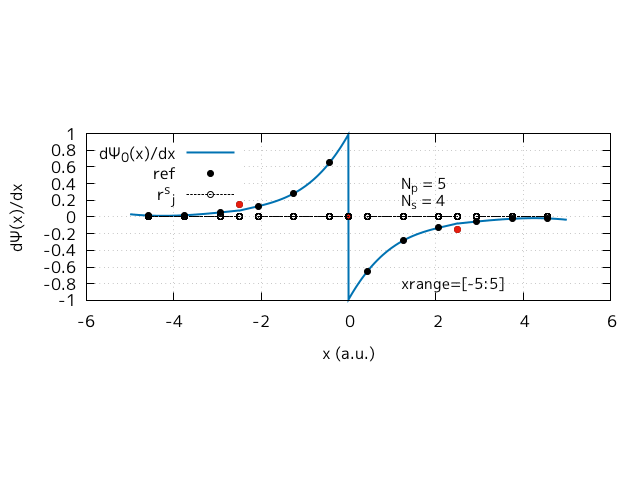
\includegraphics[scale=.22, trim={6 150 10 110},clip]{images/fedvr_deriv_wavefunc_.png} \\

%  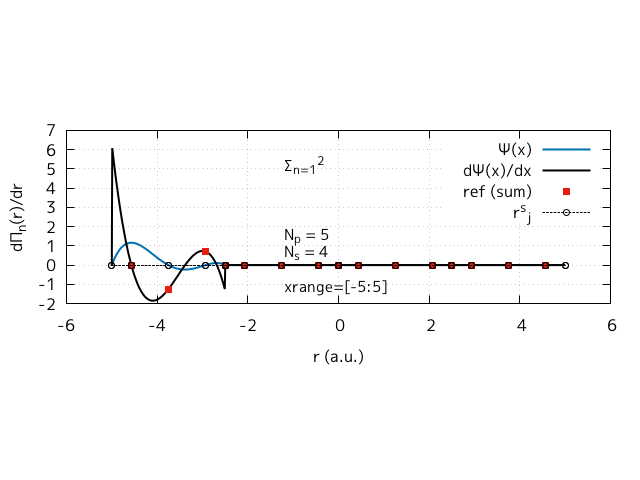
\includegraphics[scale=.20, trim={6 150 10 110},clip]{images/fedvr_sect1_dpi_diff_test_2.png} \\
%  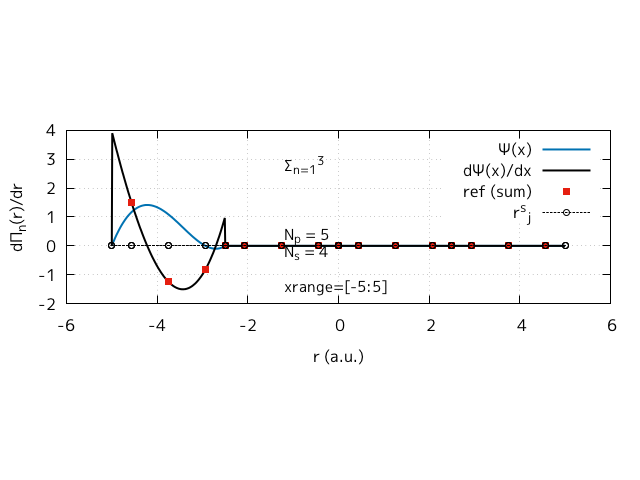
\includegraphics[scale=.20, trim={6 150 10 110},clip]{images/fedvr_sect1_dpi_diff_test_3.png} 
%  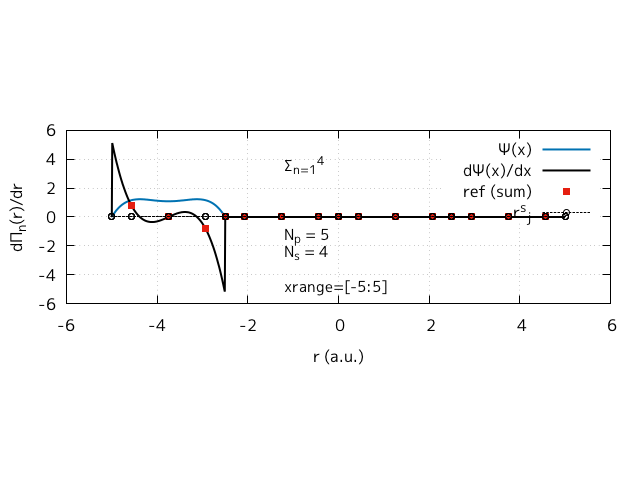
\includegraphics[scale=.20, trim={6 110 10 110},clip]{images/fedvr_sect1_dpi_diff_test_4.png} 
%%%\caption{Eigenvalues.}
%\label{fig:pemd_0114}
\end{figure}

\end{minipage}
\end{textblock*}


\begin{textblock*}{420pt}(10pt,60pt)
\footnotesize

\begin{align}
& \left.\frac{d\pi_i^s (r)}{dr}\right|_{r=r_j^s} 
       =  \frac{1}{\sqrt{\omega_i}} \left\lbrace
      \begin{array}{l} 
       \frac{1}{r_i^s - r_j^s}\prod_{\substack{k=1 \\ k\neq i,j}}^{N_p}
       \frac{r_j^s - r_k^s}{r_i^s - r_k^s}, \hspace{50pt} i \neq j, \\
       \frac{1}{2}\left(\Big[\pi_i^s(r_{N_p}^s)\Big]^2 
       - \Big[\pi_i^s(r_1^s)\Big]^2\right), \hspace{20pt} i=j,
\end{array}\right.\nonumber \\
& \frac{d\Pi_n(r)}{dr}
=  \frac{1}{\sqrt{\Omega_n}}
      \left\lbrace
         \begin{array}{l} 
       \sqrt{\omega_{N_p}^s}\,d\pi_{N_p}^s(r)/dr,  
          \hspace{10pt} \ r \leqslant r_s, \hspace{10pt} \\
       \sqrt{\omega_{1}^{s+1}}\,d\pi_{1}^{s+1}(r)/dr,  
          \hspace{10pt} r \geqslant  r_{s},
         \end{array}\right. \hspace{10pt}\mbox{with}\hspace{10pt} 
\frac{d\pi_i^s (r)}{dr}
       =  \frac{1}{\sqrt{\omega_i^s}} \sum_{\substack{j=1 \\ j\neq i}}^{N_p} 
       \frac{1}{r_i^s - r_j^s}\prod_{\substack{k=1 \\ k\neq j,i}}^{N_p}
       \frac{r - r_k^s}{r_i^s - r_k^s}, \nonumber
\end{align}

\end{textblock*}

\begin{textblock*}{300pt}(150pt,150pt)
\footnotesize
\noindent for $n = (s-1)(N_p-1) + N_p$ and reduces to $d\pi^s_i(r)/dr$ otherwise
\begin{itemize}
\item The black dots represent (\ref{eqn:disc_dpsi}) for $m=1,\ldots,N$ 
(ref)
\item The blue line represents (\ref{eqn:cont_dpsi}) in the whole range
\end{itemize}
 \begin{align}
 & \frac{d\psi(x_{m},t)}{dx} = \sum_{n=1}^{N} \sqrt{\omega^s_i}
           c_n(t)\frac{d\Pi_n(x_{m})}{dx} \label{eqn:disc_dpsi}\\
 & \frac{d\psi(x,t)}{dx} = \sum_{n=1}^{N} \sqrt{\omega^s_i}
           c_n(t)\frac{d\Pi_n(x)}{dx} \label{eqn:cont_dpsi}
 \end{align}


\end{textblock*}



\begin{textblock*}{200pt}(10pt,220pt)
\footnotesize
\color{red}{The values for $n^\prime = (s-1)(N_p-1)+N_p$ are off}
\end{textblock*}

\end{frame}





\begin{frame}
\frametitle{Quantum theory of radiation by nonstationary systems 
	with application to high-order harmonic generation
        (Phys. Rev. A 101, 013410 (2020))}
	\framesubtitle{The FEDVR basis - Extension by continuity}

\begin{textblock*}{100pt}(5pt,60pt)
%\centering
%\rotatebox{90}{
 \begin{minipage}{0.0\linewidth}
 \begin{figure}[tp]
 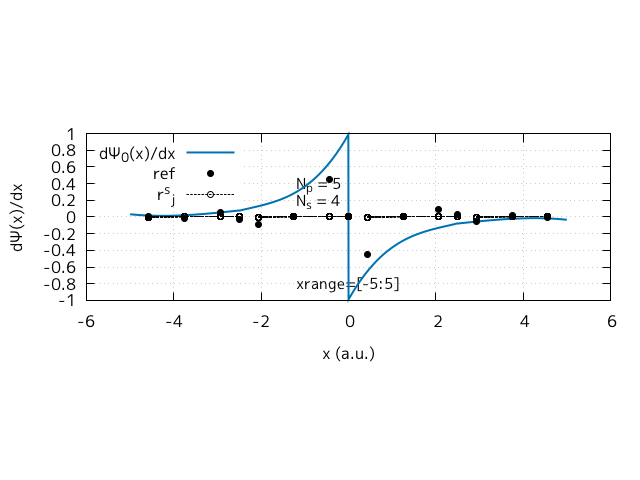
\includegraphics[scale=.25, trim={6 150 10 110},clip]{images/fedvr_deriv_wavefunc_1.png} \\
 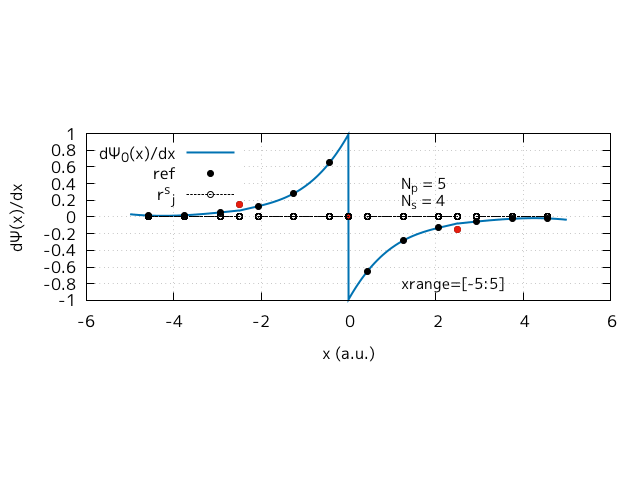
\includegraphics[scale=.25, trim={6 150 10 110},clip]{images/fedvr_deriv_wavefunc_.png} \\
 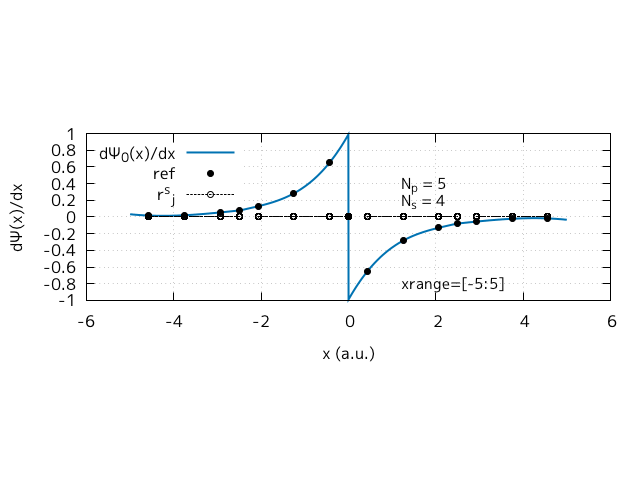
\includegraphics[scale=.25, trim={6 100 10 110},clip]{images/fedvr_deriv_wavefunc_fix.png}
%%%\caption{Eigenvalues.}
%\label{fig:pemd_0114}
\end{figure}

\end{minipage}
\end{textblock*}


\begin{textblock*}{200pt}(250pt,130pt)
%\centering
%\rotatebox{90}{

\begin{itemize}
\footnotesize
\item (Up) What was shown last week
\item (Middle) Improvement of the discrete formula
\item (Down) Fixing the values at the boundaries
\end{itemize}


\end{textblock*}


%%\begin{textblock*}{100pt}(255pt,60pt)
%%%\centering
%%%\rotatebox{90}{
%% \begin{minipage}{0.0\linewidth}
%% \begin{figure}[tp]
%% 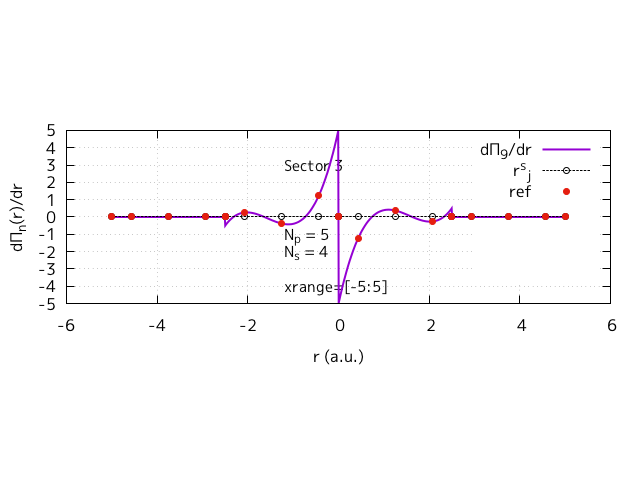
\includegraphics[scale=.20, trim={6 150 10 110},clip]{images/fedvr_sect3_dpi_diff_1.png} \\
%%  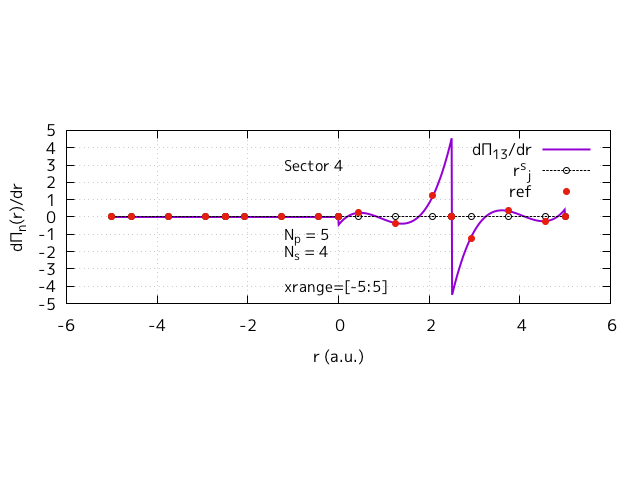
\includegraphics[scale=.20, trim={6 150 10 110},clip]{images/fedvr_sect4_dpi_diff_1.png} \\
%%% 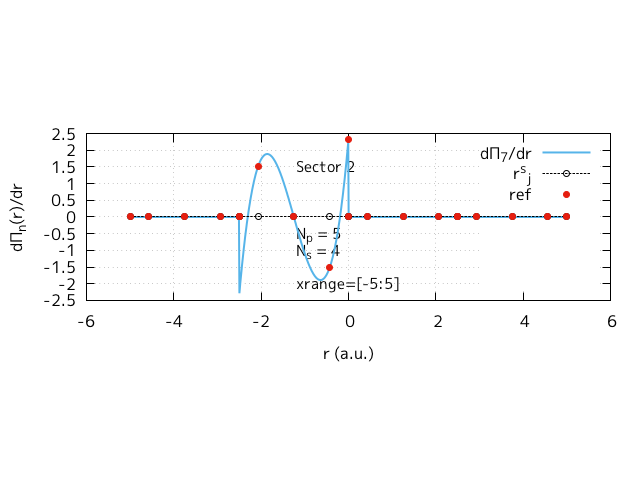
\includegraphics[scale=.20, trim={6 150 10 110},clip]{images/fedvr_sect2_dpi_diff_3.png} 
%%% 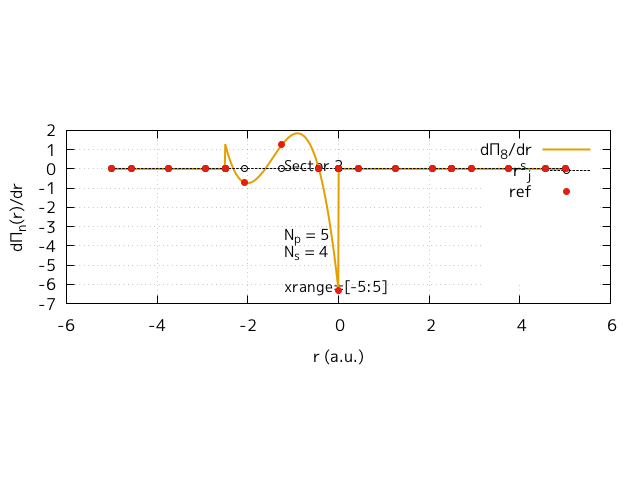
\includegraphics[scale=.20, trim={6 110 10 110},clip]{images/fedvr_sect2_dpi_diff_4.png} 
%%%%%\caption{Eigenvalues.}
%%%\label{fig:pemd_0114}
%%\end{figure}
%%
%%\end{minipage}
%%\end{textblock*}
%
%
%%\begin{textblock*}{\linewidth}(90pt,60pt)
%%\rotatebox{0}{
%%\begin{minipage}{\linewidth}
%%{
%%\Tiny
%%\centering
%%\input{tables/rk_4_5.tab}
%%}
%%\end{minipage}
%%}
%%\end{textblock*}



\end{frame}






















%\begin{frame}
%\frametitle{Quantum theory of radiation by nonstationary systems 
%	with application to high-order harmonic generation
%        (Phys. Rev. A 101, 013410 (2020))}
%	\framesubtitle{The wavefunction $\phi_\omega(x,t) \;\;\;(\omega=1)$}
%
%\begin{textblock*}{500pt}(5pt,60pt)
%%\centering
%%\rotatebox{90}{
% \begin{minipage}{0.0\linewidth}
% \begin{figure}[tp]
% 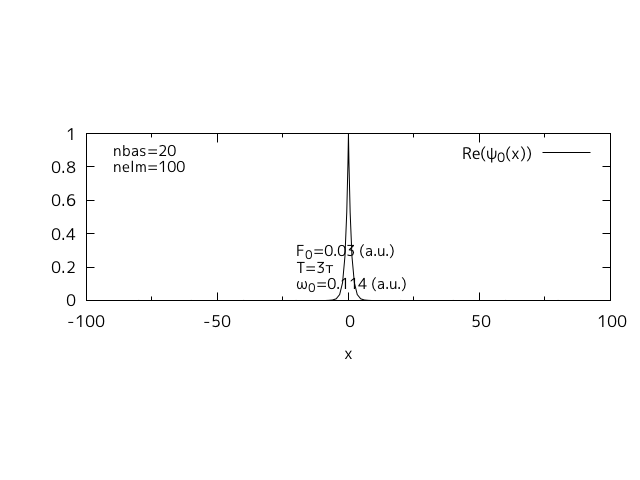
\includegraphics[scale=.20, trim={6 100 0 133},clip]{images/114_f003_3_03_wfc0.png} \\
% 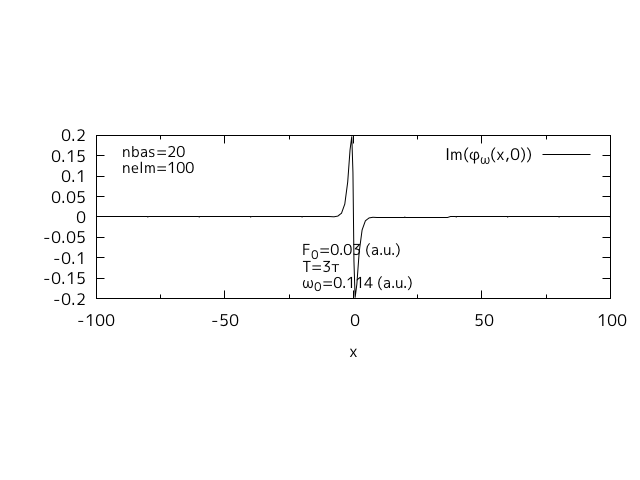
\includegraphics[scale=.20, trim={6 100 0 130},clip]{images/114_f003_3_03_phic0.png} \\
%% \includegraphics[scale=.20, trim={6 130 10 130},clip]{images/114_f003_8_03_hhg.png} 
%%%\caption{Eigenvalues.}
%%\label{fig:pemd_0114}
% \end{figure}
%
%\end{minipage}
%\end{textblock*}
%
%
%\begin{textblock*}{500pt}(130pt,60pt)
%%\centering
%%\rotatebox{90}{
% \begin{minipage}{0.0\linewidth}
% \begin{figure}[tp]
% 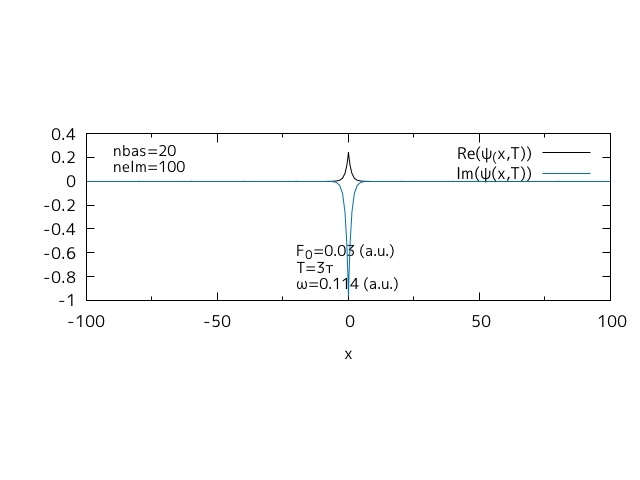
\includegraphics[scale=.20, trim={6 100 0 133},clip]{images/114_f003_3_03_wfc.png} \\
% 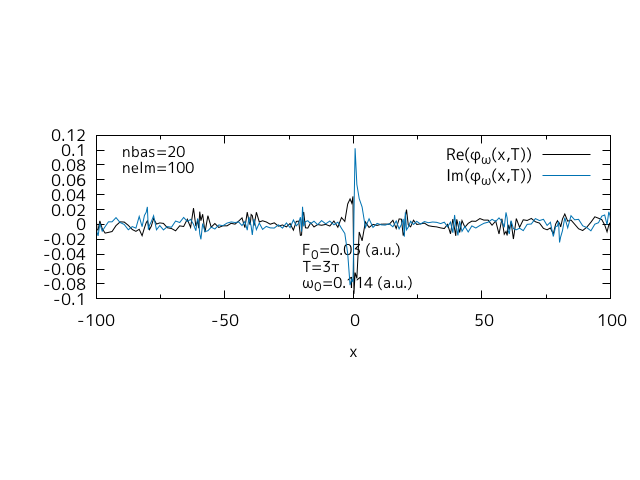
\includegraphics[scale=.20, trim={6 100 0 130},clip]{images/114_f003_3_03_phic.png} \\
%% 
\includegraphics[scale=.20, trim={30 130 10 130},clip]{images/114_f003_12_07_hhg.png} 
%%%\caption{Eigenvalues.}
%%\label{fig:pemd_0114}
% \end{figure}
%
%\end{minipage}
%\end{textblock*}
%
%
%\begin{textblock*}{500pt}(255pt,60pt)
%%\centering
%%\rotatebox{90}{
% \begin{minipage}{0.0\linewidth}
% \begin{figure}[tp]
% 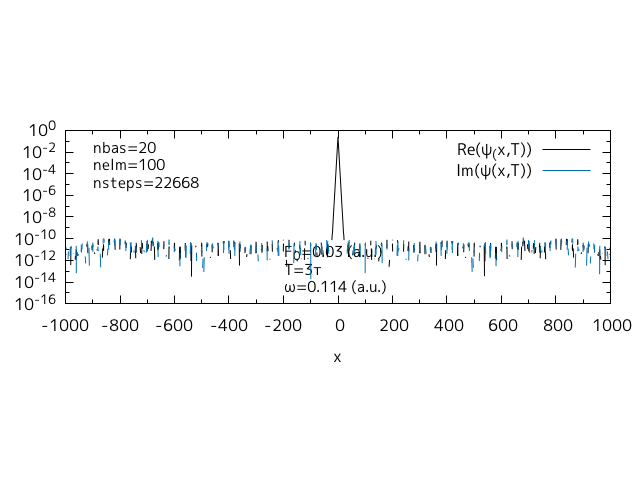
\includegraphics[scale=.20, trim={6 100 0 133},clip]{images/114_f003_3_03_wfc_log.png} \\
% 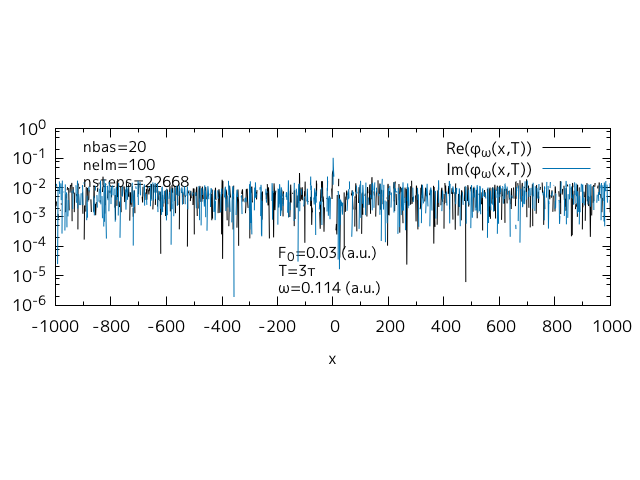
\includegraphics[scale=.20, trim={6 100 0 130},clip]{images/114_f003_3_03_phic_log.png} \\
% 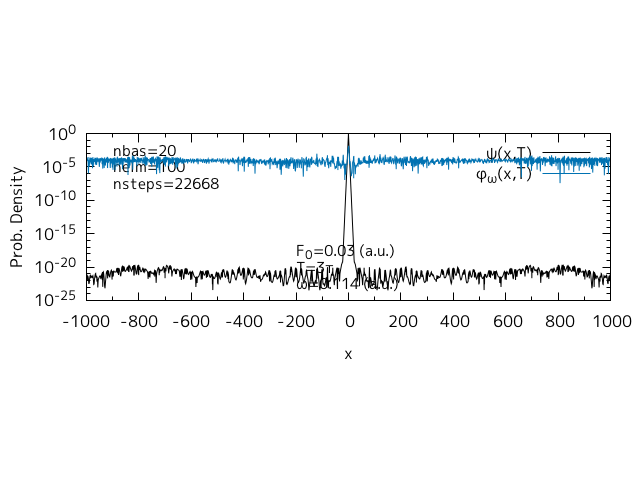
\includegraphics[scale=.20, trim={6 100 0 130},clip]{images/114_f003_3_03_density.png} 
%%%\caption{Eigenvalues.}
%%\label{fig:pemd_0114}
% \end{figure}
%
%\end{minipage}
%\end{textblock*}
%
%
%\begin{textblock*}{400pt}(30pt,200pt)
%\footnotesize
%\begin{itemize}
%\item Laser switched off
%\end{itemize}
%
%\end{textblock*}
%
%
%
%\end{frame}







%\begin{frame}
%\frametitle{Quantum theory of radiation by nonstationary systems 
%	with application to high-order harmonic generation
%        (Phys. Rev. A 101, 013410 (2020))}
%	\framesubtitle{Correct approach}
%
%
%\begin{textblock*}{400pt}(30pt,50pt)
%\footnotesize
%\begin{align}
%  Q_\nu = \alpha^2 \sum_n \left| b_{n\nu}\right|^2 
%\end{align}
%\end{textblock*}
%
%
%\begin{textblock*}{400pt}(30pt,80pt)
%\footnotesize
%\begin{align}
%b_{n\nu}(t\geqslant T) & = b_{n\nu} 
%   + i e^{i(E_n+\omega)t}\langle \psi_n^-|\hat{R}_\nu|\psi(t)\rangle
%\end{align}
%\end{textblock*}
%
%
%
%\begin{textblock*}{400pt}(30pt,100pt)
%\footnotesize
%\begin{align}
%\hat{R}_\nu = \int_0^\infty e^{i\hat{H}_a t}\boldsymbol{A}_\nu
%\hat{\boldsymbol{\rm p}}
%e^{-i\hat{H}_a t} e^{i\omega t - \epsilon t} dt
%\end{align}
%\end{textblock*}
%
%
%\begin{textblock*}{400pt}(30pt,150pt)
%\footnotesize
%\begin{align}
%|\psi(t)\rangle = \sum_n a_n(t) e^{-E_n t}|\psi_n^-\rangle, \\
%|\phi_\nu(t)\rangle = \sum_n b_{n\nu}(t) e^{-E_n t}|\psi_n^-\rangle
%\end{align}
%\end{textblock*}
%
%
%\begin{textblock*}{400pt}(30pt,200pt)
%\footnotesize
%%\begin{itemize}
%%\item How to deduce the coefficients of $\phi_\nu$?
%\begin{align}
%\left.\langle\psi(t)|\phi_\nu(t)\rangle\right|_{t\geqslant T} 
%= \sum_n a_n^*(T) b_{n\nu}(T)
%= -i\boldsymbol{\rm A}_\nu \boldsymbol{\rm p}(\omega), 
%\end{align}
%%\end{itemize}
%\end{textblock*}
%
%
%
%\end{frame}



%\begin{frame}
%\frametitle{Quantum theory of radiation by nonstationary systems 
%	with application to high-order harmonic generation
%        (Phys. Rev. A 101, 013410 (2020))}
%	\framesubtitle{Resolution}
%
%
%\begin{textblock*}{400pt}(30pt,50pt)
%\footnotesize
%\begin{align}
%  Q_\nu = \alpha^2 \sum_n \left| b_{n\nu}\right|^2 
%\end{align}
%\end{textblock*}
%
%
%\begin{textblock*}{400pt}(30pt,80pt)
%\footnotesize
%\begin{align}
%b_{n\nu}(t\geqslant T) & = b_{n\nu} 
%   + i e^{i(E_n+\omega)t}\langle \psi_n^-|\hat{R}_\nu|\psi(t)\rangle
%\end{align}
%\end{textblock*}
%
%
%
%\begin{textblock*}{400pt}(30pt,100pt)
%\footnotesize
%\begin{align}
%\hat{R}_\nu = \int_0^\infty e^{i\hat{H}_a t}\boldsymbol{A}_\nu
%\hat{\boldsymbol{\rm p}}
%e^{-i\hat{H}_a t} e^{i\omega t - \epsilon t} dt
%\end{align}
%\end{textblock*}
%
%
%\begin{textblock*}{400pt}(30pt,150pt)
%\footnotesize
%\begin{align}
%|\psi(t)\rangle = \sum_n a_n(t) e^{-E_n t}|\psi_n^-\rangle, \\
%|\phi_\nu(t)\rangle = \sum_n b_{n\nu}(t) e^{-E_n t}|\psi_n^-\rangle
%\end{align}
%\end{textblock*}
%
%
%\begin{textblock*}{400pt}(30pt,200pt)
%\footnotesize
%%\begin{itemize}
%%\item How to deduce the coefficients of $\phi_\nu$?
%\begin{align}
%\left.\langle\psi(t)|\phi_\nu(t)\rangle\right|_{t\geqslant T} 
%= \sum_n a_n^*(T) b_{n\nu}(T)
%= -i\boldsymbol{\rm A}_\nu \boldsymbol{\rm p}(\omega), 
%\end{align}
%%\end{itemize}
%\end{textblock*}
%
%
%
%\end{frame}
